\documentclass[UTF8]{ctexart}
\usepackage{amsmath}
\usepackage{cases}
\usepackage{cite}
\usepackage{graphicx}
\usepackage[margin=1in]{geometry}
\geometry{a4paper}
\usepackage{float}
\usepackage{array}
\usepackage{multirow}
\usepackage{fancyhdr}
\usepackage{listings}

\usepackage[colorlinks=true, urlcolor=blue, linkcolor=black]{hyperref}
\pagestyle{fancy}
\fancyhf{}
\setlength{\parindent}{0pt}


\title{利用扭摆测量转动惯量与剪切模量}
\author{郑之浩 \thanks{github.com/alizeisnotalize/physics-experiment}}
\date{\today}
\pagenumbering{arabic}

\begin{document}

\fancyhead[L]{郑之浩}
\fancyhead[C]{利用扭摆测量转动惯量与剪切模量}
\fancyfoot[C]{\thepage}

\maketitle
\tableofcontents
\newpage

\section{摘要}
剪切模量定义为切应力与切应变之比，刻画了材料抵抗剪切形变的能力，是工程结构
设计、材料力学性能评估及固体物理研究中的重要参数。扭摆是通过扭转弹性细丝储存弹性
势能的机械振子，被广泛应用于精确测量材料的剪切模量与刚体的转动惯量。值得一提的是，
上世纪 40 年代，中国物理学家葛庭燧在扭摆原理基础上，发明了用于测量金属内耗的专用
装置——葛氏摆。该装置通过定量测量扭摆振动过程中振幅的衰减速率，可精准表征扭丝材
料内部的能量耗散特性（即内耗），为研究金属晶体缺陷、相变及力学阻尼行为提供了极具
价值的实验手段。

\section{实验目的}
\noindent 1. 了解扭摆的工作原理； \newline
2. 掌握扭摆系统测量材料剪切模量和刚体转动惯量的方法； \newline
3. 练习PASCO数字化实验平台的使用。\newline


\section{实验仪器}

\noindent 扭摆、PASCO 数字化实验平台（包括850接口与Capstone 软件）、待测圆环、电子天
平、螺旋测微器、游标卡尺、钢卷尺等。 \newline
PASCO 数字化实验平台是一个集成了传感器、数据采集器和计算机软件的实验系统，能够实现对各种物理量的实时测量和数据分析。该平台通过传感器将物理量转换为电信号，并通过数据采集器将信号传输到计算机软件中进行处理和分析。
\begin{figure}[htbp]
  \centering
  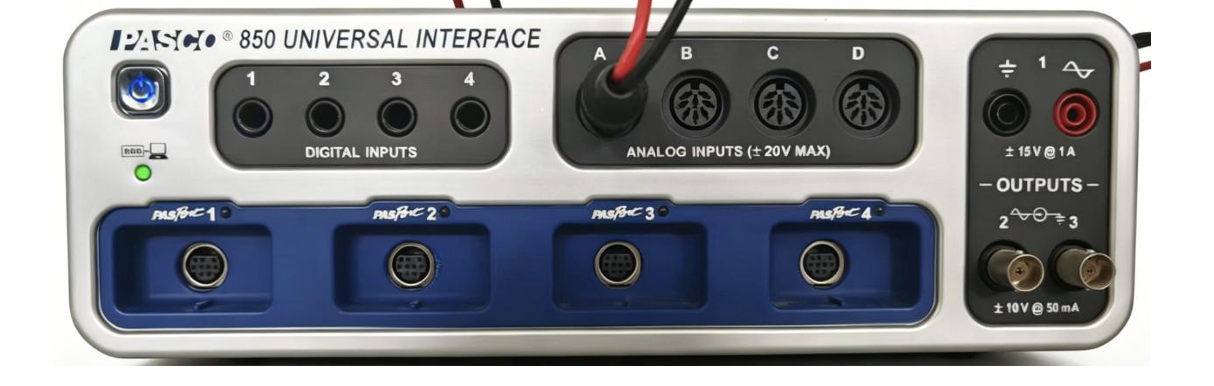
\includegraphics[width=0.6\textwidth]{PascoF850.png}
  \caption{PascoF850}
  \label{fig:example}
\end{figure}

\begin{figure}[htbp]
  \centering
  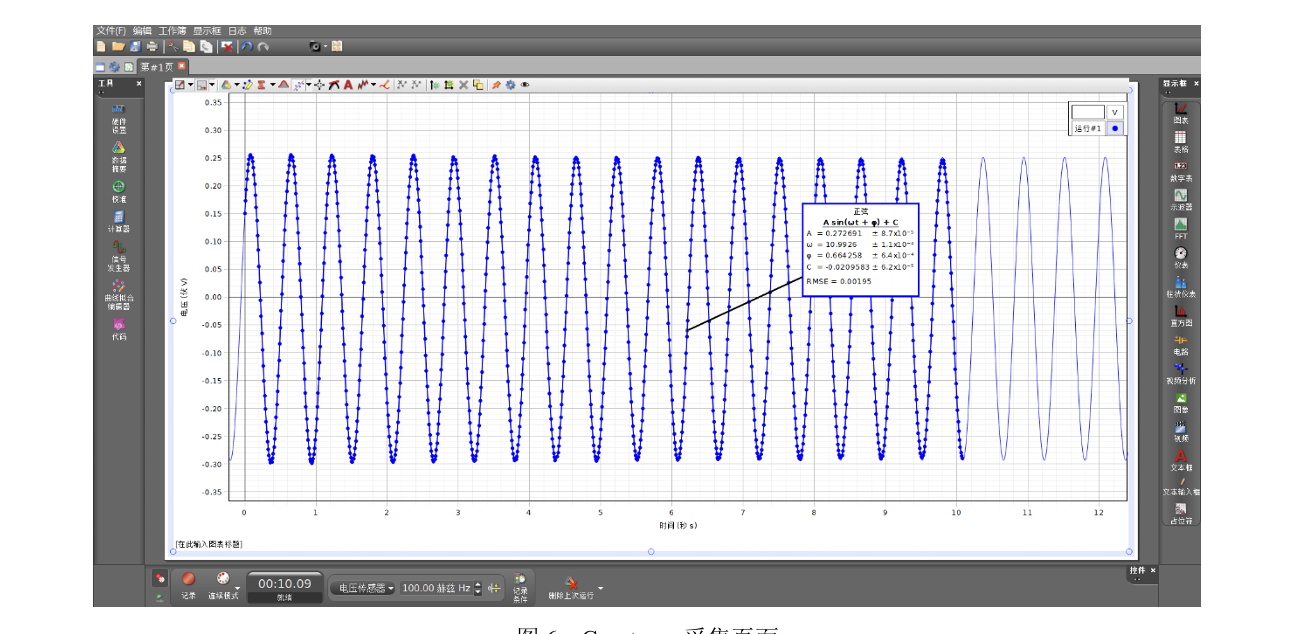
\includegraphics[width=0.6\textwidth]{PascoCapstone.png}
  \caption{PascoCapstone}
  \label{fig:capstone}
\end{figure}


\noindent 扭摆装置由扭转弹性细丝、刚体和支架组成。扭转弹性细丝用于储存弹性势能，刚体用于测量转动惯量，支架用于固定装置。通过扭转弹性细丝的扭转角度和振动周期，可以计算出材料的剪切模量和刚体的转动惯量。
\begin{figure}[htbp]
  \centering
  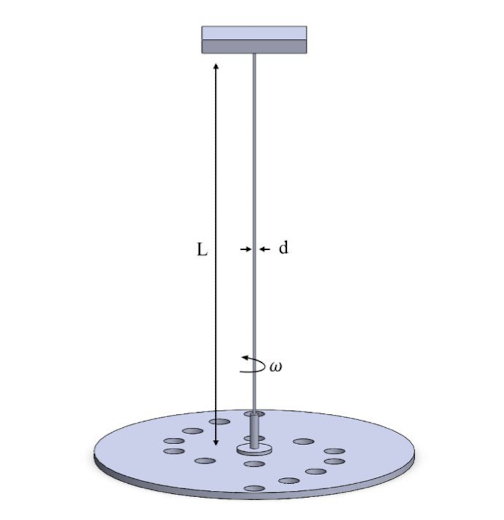
\includegraphics[width=0.6\textwidth]{扭摆.png}
  \caption{扭摆装置}
  \label{fig:torsion_pendulum}
\end{figure}

\section{实验原理}

\subsection{剪切模量}

\begin{figure}[htbp]
  \centering
  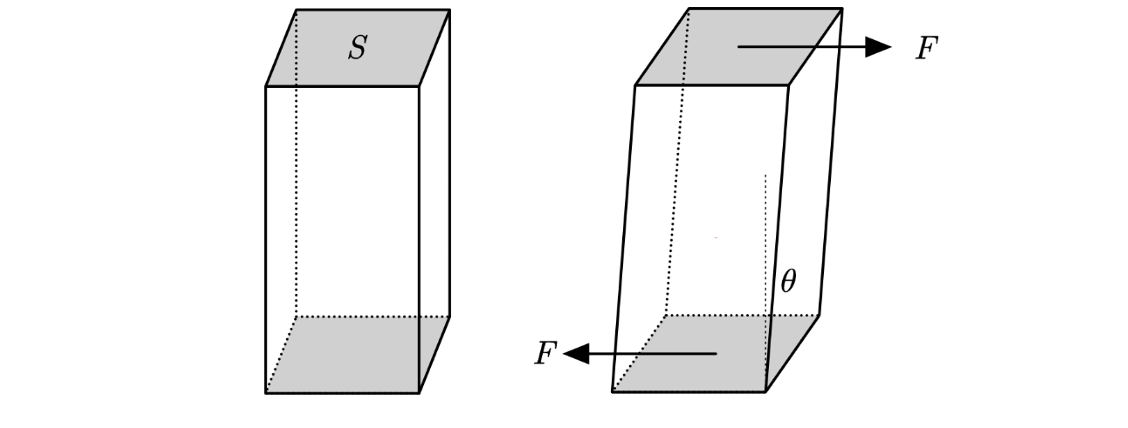
\includegraphics[width=0.6\textwidth]{剪切模量.png}
  \caption{剪切模量示意图}
  \label{fig:shear_modulus}
\end{figure}

\noindent 考虑材料中一块长方体的微元（图1）。在长方体的上、下底面施加一对方向在底面内的
力偶。在弹性力学中，单位面积上受到的面内方向的力称为切应力（shear stress），即：

\begin{equation}
  \tau = \frac{F}{A} 
\end{equation}
在切应力下，微元上、下底面将发生相对滑动。称垂直于底面的棱相对平衡状态转过的角度 $\theta$ 为切应变（shear strain），。在弹性范围内，$\tau$ 与 $\theta$ 称正比，比例系数称为切变模量（shear modulus），
即： 
\begin{equation}
  \mu  = \frac{\tau}{\theta} = \frac{F/A}{\theta} 
\end{equation}
可以证明，切应变存储的弹性势能密度为：
\begin{equation}
  \varepsilon  = \frac{1}{2}\mu \theta^2
\end{equation}

\subsection{扭摆}
扭摆的结构如图2所示，其中扭丝上端固定不动，下端与一个刚体（称为摆盘）固定。
当摆盘相对平衡位置转动小角度$\theta$，扭丝会产生恢复力矩。在弹性形变范围内,$T $与$\theta$成正比，即：

\begin{equation}
  T = -k\theta
\end{equation}

其中$k$为扭转系数，单位为N·m/rad。下面分析$k$与扭丝的剪切模量以及几何尺寸的关系。\newline
\noindent 下图为扭丝形变的放大示意图，图中P点位于扭丝的上端面。考虑在自由状态时经过P
点，且与扭丝的中轴线平行的直线。当扭丝下端面相对静止状态扭转小角度$\theta$时，这条直线
转过的角度为：

\begin{equation}
  \phi = \frac{r\theta}{L}
\end{equation}

其中$L$为扭丝的长度，$r$为P点到扭丝中轴线的距离。根据定义，$\phi$就是P点的切应变。对应的切应力为：

\begin{equation}
  \tau = \mu \phi = \mu \frac{r\theta}{L}
\end{equation}

扭丝上端面距离中心为$r$到$r+dr$的环面受到的力矩为：

\begin{equation}
  dT = \tau \cdot 2\pi r dr \cdot r = 2\pi \mu \frac{r^3\theta}{L} dr
\end{equation}

因此扭丝受到总力矩为： 

\begin{equation}
  T = \int_0^{\frac{d}{2}} dT = \frac{\pi \mu d^4}{32L} \theta
\end{equation}

因此有关系：

\begin{equation}
  k = \frac{\pi \mu d^4}{32L}
\end{equation}

上式也可以根据弹性势能得到。根据（3）式，扭丝储存的弹性势能为： 
\begin{equation}
  E = \int_0^{\frac{d}{2}} \varepsilon \cdot 2\pi r dr \cdot L = \frac{\pi \mu d^4}{64L} \theta^2
\end{equation}

对比$E_k = \frac{1}{2}k\theta^2$，可得$k = \frac{\pi \mu d^4}{32L}$，可以得到（9）式。
\noindent 根据刚体定轴转动定律，扭摆在平衡位置附近的运动方程为：

\begin{equation}
  I\frac{d^2\theta}{dt^2} = -k\theta
\end{equation}

其中$I$为摆盘的转动惯量。因此摆盘在平衡位置做简谐振动，角频率为：

\begin{equation}
  \omega = \sqrt{\frac{k}{I}}
\end{equation}

\subsection{扭摆的测量原理}
\noindent 为了测量扭摆的扭力系数$k$，在摆盘上对称地固定两个形状、质量相同的球（或其它具
有旋转对称性的物体）。设每个小球的质量为$m$，小球质心到扭丝的距离为$r$，则此时扭摆运
动部分的转动惯量增加为:

\begin{equation}
  I_d = I + \frac{4}{5}mr^2 + 2md^2 = I_0 + 2md^2
\end{equation}

由（12）式可知，此时扭摆的角频率$\omega_d$与$d$满足关系：

\begin{equation}
  \frac{1}{\omega_d^2} = \frac{I_0 + 2md^2}{k}
\end{equation}

\noindent 实验中改变$d$，测量对应的$\omega_d$，根据这个关系做直线拟合，就可以得到$k$和$I_0$。测出扭丝的直
径与长度，根据（9）式可得扭丝材料的剪切模量为：

\begin{equation}
  \mu = \frac{32kL}{\pi d^4}
\end{equation}

测出不放小球（即空载）时扭摆的角频率$\omega_0$，可得摆盘转动惯量为：

\begin{equation}
  I_0 = \frac{k}{\omega_0^2}
\end{equation}

将待测物体放置在扭摆上，测量扭摆的振动角频率$\omega'$，则待测物体的转动惯量为：

\begin{equation}
  I_m = k(\frac{1}{\omega^2} - \frac{1}{\omega'^2})
\end{equation}

\section{实验内容}

\noindent 1. 测量扭摆的参数（扭丝的长度、直径，小球的质量和直径）； \\
\noindent 2. 测量小球放在不同位置时的扭摆频率，计算扭丝的扭力系数和剪切模量；\\ 
3. 测量小球和待测圆环的转动惯量。

\section{实验方法}

\noindent 本实验所用摆盘为直径125mm、厚度2mm的铝制圆盘，上面对称分布7对直径12mm的圆
孔，圆孔中心到摆盘中心的距离分别为20mm、25mm、30mm、35mm、40mm、45mm和50mm
。这些圆孔用来摆放小球，定量改变转动惯量。摆盘通过螺丝与扭丝的下夹头固定在
一起。为了测量摆角，在扭丝的上夹头与之间之间安装了一个扭矩传感器，其作用是将摆丝
受到的扭矩转换为电信号。用电压传感器将扭矩传感器的信号输出接入PASCO850接口的模
拟输入端（一共有4各，任选一个）。\newline


\noindent 打开Capstone 软件，在硬件设置窗口将输入模拟端口设置为“电压传感器”(在下拉菜
单中选择)。从软件按界面的右侧新建一个给图表，纵坐标选择为前面添加的电压传感器，
横坐标设为“时间（秒s）”，设置合适的采样率（比如50或100Hz），点击“记录”按钮，
就可以采集到电压传感器的波形。使用软件自带的拟合工具，选用“正弦："$Asin(\omega t  + \varphi )+ C$"模型拟合采集波形，即可得到扭摆振动的角频率。注意，程序给出的最
佳拟合值的有效位数可能不够多。以图2中的情况为例，$\omega$ 的不确定度为$1.1×10^−4$，因此
$\omega$应该保留4到5位小数。而程序默认只保留4位有效数字。这时需要点击拟合信息框，调
出“曲线拟合属性”窗口，修改系数的数字格式

\begin{figure}[htbp]
  \centering
  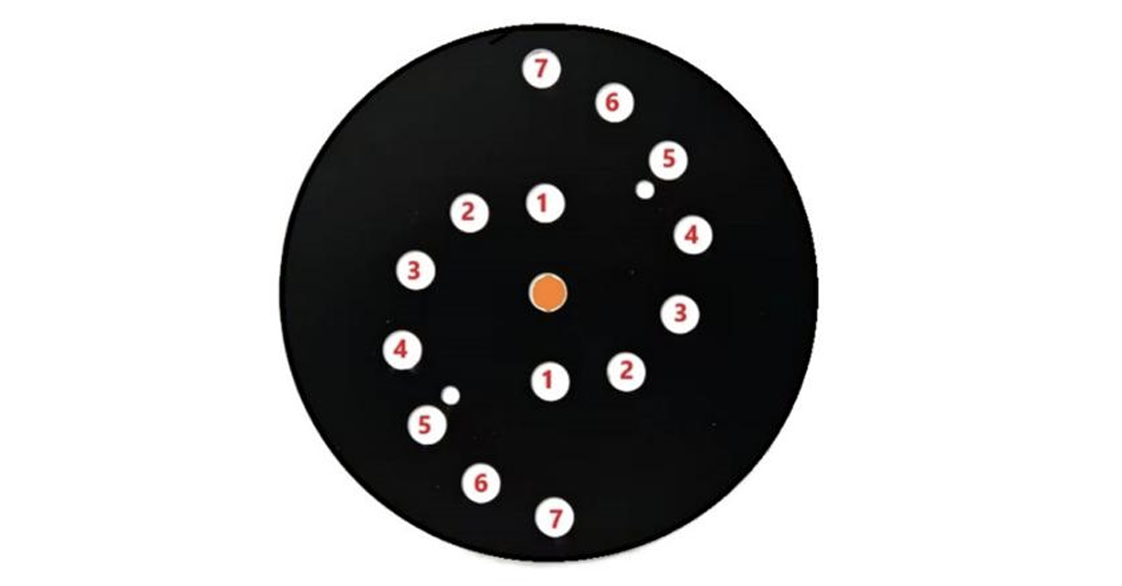
\includegraphics[width=0.6\textwidth]{摆盘俯视图.png}
  \caption{摆盘俯视图}
  \label{fig:example}
\end{figure}

\section{注意事项}

\noindent 1. 安装/拆卸摆盘时需要用一只手拿扳手固定下夹头，另一只手拧固定螺丝。过程中要尽量减
小扭丝的弯曲和扭动角度。 \\
\noindent 2. 测量扭摆周期时，摆盘的初始角度不要过大，大约10度即可。摆角过大可能会使铜球不稳
定，也可能引入扭矩的非线性。

\section{实验数据与结果}

\subsection{装置测量参数}

\noindent 刚体

\begin{table}[H]
\centering
\begin{tabular}{|>{\raggedright\arraybackslash}p{3.9cm}|>{\raggedright\arraybackslash}p{4.5cm}|>{\raggedright\arraybackslash}p{4.6cm}|>{\raggedright\arraybackslash}p{4.7cm}|}
\hline
小球质量($g$) & $m_1 = 35.07g$     & $m_2 = 35.07g$     & 平均$m = 35.07g$   \\ \hline
圆环        & 内径$d_1 = 5.344 mm$ & 外径$d_2 = 7.660 mm$ & 质量$M = 468.16 g$ \\ \hline
\end{tabular}
\end{table}
\noindent 圆环转动惯量计算值

\begin{equation}
  I_cal = \frac{M}{8}(d_1^2 + d_2^2) = 0.0003 kg·m^2
\end{equation}

\noindent 扭丝

\begin{table}[H]
\centering
\begin{tabular}{|>{\centering\arraybackslash}p{5.9cm}rrrrrl|}
\hline
\multicolumn{7}{|c|}{长度$L = 443.2 mm$}                                                                                                                                                                                                                             \\ \hline
\multicolumn{1}{|>{\centering\arraybackslash}p{5.9cm}|}{\multirow{2}{=}{直径$D(mm)$}} & \multicolumn{1}{r|}{1}     & \multicolumn{1}{r|}{2}     & \multicolumn{1}{r|}{3}     & \multicolumn{1}{r|}{4}     & \multicolumn{1}{r|}{5}     & 平均                          \\ \cline{2-7} 
\multicolumn{1}{|>{\centering\arraybackslash}p{5.9cm}|}{}                           & \multicolumn{1}{r|}{$1.405$} & \multicolumn{1}{r|}{$1.403$} & \multicolumn{1}{r|}{$1.402$} & \multicolumn{1}{r|}{$1.404$} & \multicolumn{1}{r|}{$1.402$} & \multicolumn{1}{r|}{$1.4032$} \\ \hline
\end{tabular}
\end{table}

\subsection{改变小球的位置($d$),测量扭摆的角频率($\omega$)}

\begin{table}[H]
\centering
\begin{tabular}{|>{\raggedright\arraybackslash}p{6.7cm}|l|l|l|l|l|l|l|}
\hline
$d(mm)$                  & \multicolumn{1}{r|}{20} & \multicolumn{1}{r|}{25} & \multicolumn{1}{r|}{30} & \multicolumn{1}{r|}{35} & \multicolumn{1}{r|}{40} & \multicolumn{1}{r|}{45} & \multicolumn{1}{r|}{50} \\ \hline
$\omega (rad/s)$ & $21.3319$               & $20.2689$               & $19.1649$               & $18.0733$               & $17.0080$               & $16.0076$               & $15.0752$               \\ \hline
\end{tabular}
\end{table}

\begin{figure}[H]
  \centering
  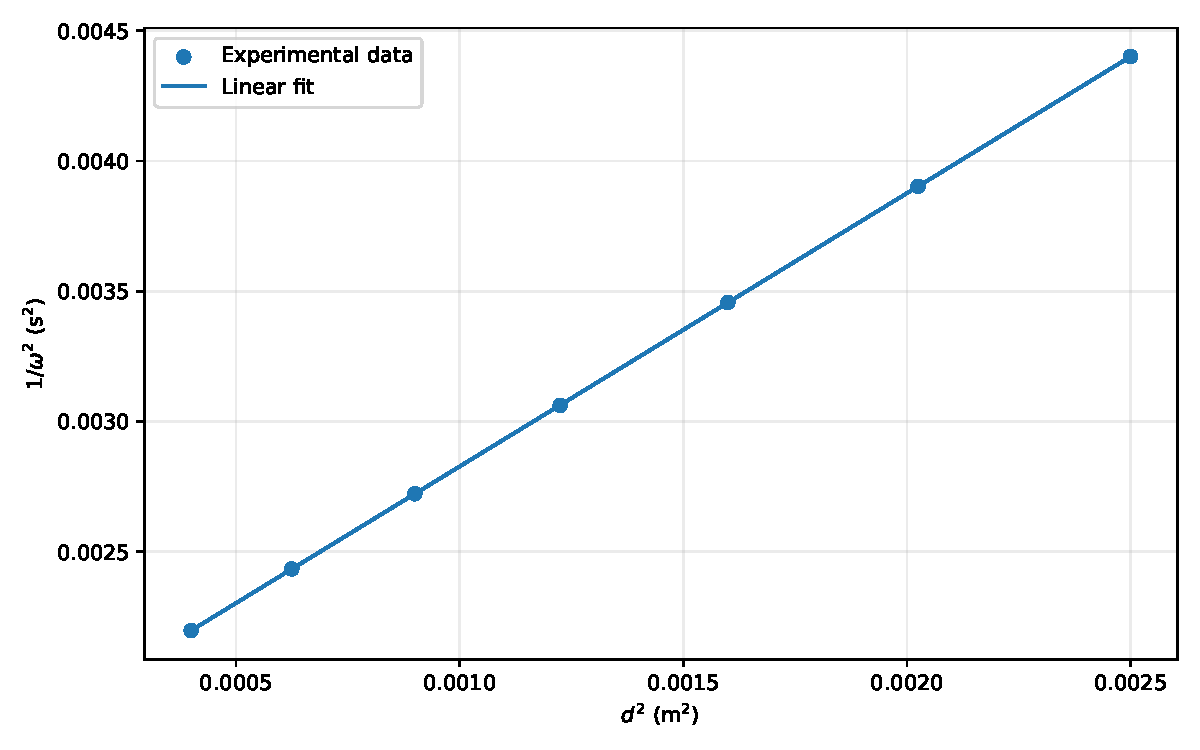
\includegraphics[width=0.6\textwidth]{results2/fit.pdf}
  \caption{拟合图像}
\end{figure}

\noindent 拟合直线关系$\frac{1}{\omega^2} = a d^2 + b$, 得$a = 1.0489{ } b = 0.0018$,决定系数$R^2 = 0.9999$\newline
\noindent 扭力系数$k = \frac{2m}{a} = 0.0669 N·m/rad$，摆盘转动惯量$I_0 = \frac{b}{a} = 0.0017 kg·m^2$\newline
\noindent 计算剪切模量$\mu = \frac{32kL}{\pi d^4} = 7.9 \times 10^{10} Pa$，与钢的剪切模量相符。

\subsection{测量扭摆空载角频率($\omega$)和负载角频率($\omega‘$)，计算圆环的转动惯量}

\begin{table}[H]
\centering
\begin{tabular}{|>{\raggedright\arraybackslash}p{4.8cm}|l|r|r|>{\raggedright\arraybackslash}p{4cm}|}
\hline
                  & \multicolumn{1}{r|}{1} & 2       & 3       & 平均        \\ \hline
$\omega (rad/s)$  & $24.0040$              & 24.0048 & 24.0063 & $24.0050$ \\ \hline
$\omega '(rad/s)$ & $10.3100$              & 10.3141 & 10.3106 & $10.3115$ \\ \hline
\end{tabular}
\end{table}

\noindent 转动惯量测量值

\begin{equation}
  I_mes = k(\frac{1}{\omega^2} - \frac{1}{\omega'^2}) = 0.0003 kg·m^2
\end{equation}

\noindent 测量值与理论值的相对误差：

\begin{equation}
  \delta = \frac{I_{\mathrm{mes}} -I_{\mathrm{cal}}}{I_{\mathrm{cal}}} = 0.56\%
\end{equation}

\section{正片开始（）}

\subsection{稍微更准确的讨论}

\noindent 害害害,zzh觉得这个bnu实验手册的理论太简单了，于是决定加一点点细节（）\newline
\noindent 显然嗷，这个扭摆并非理想的简谐振子，存在阻尼。由我们小学二年级就学过的阻尼振动知识非常容易知道嗷，这个实际的运动方程不应该是仅仅一个正（余）弦函数那么easy啊。
而是应该e指数和正（余）弦的叠加。假如你正好很闲把测量时间拉长了一丢丢，那就很容易观察到嗷，振幅是不断衰减的。\newline
\noindent 于是我们就有了一个更准确的运动方程：

\begin{equation}
  u = A e^{-\beta t} \cos(\omega t + \varphi)
\end{equation}

\noindent 不过嘞，即使是对于这个理想的运动方程，我们依然做了理想化的假设：\newline

\begin{centering}
  1、低速情况下摆受到的阻力与速度成正比 \newline
  2、小角度情况下，摆线不发生塑性形变，回复力矩和角度成正比（即能量耗散仅仅因为空气阻力）\newline
  3、摆线不随着实验的进行发生金属疲劳\newline
  4、实验正确进行，扭摆仅仅在xOy平面内转动，不是发生了三维空间的球面摆运动
\end{centering}

\noindent   \newline
\noindent 这个时候就有闲着没事干的朋友有意见了，他说：“oi，zzh。如果摆受到的空气阻力和速度高阶成正比呢？你是如何确定剩余条件满足理想情况嘞？”\newline

\noindent 这个问题非常好嗷。zzh也想过这个问题。对于第一个问题我的回答是经过我马后炮的拟合我发现一阶情况下决定系数已经能达到三个9了，故采用阻力与速度一阶成正比的模型应该是没问题的。对于第二个问题，经过我的估算这些非理想因素带来的误差数量级小于实验中A类和B类误差合成后的数量级，故也可以忽略。\newline

\noindent By the way,估计误差的数量级并确定依此影响因素是非常重要的技能（）如果打pt就会知道要是你一心想着做个very beautiful的模型你会算死的（） 

\subsection{处理数据}

\noindent OK啊,现在我们开始这个实验最恶心的部分 \newline
\noindent 其实在Pasco Captone软件中是可以直接拟合的。但是对于形如$ u = A e^{-\beta t} \cos(\omega t + \varphi)$这种初等函数的复合，我们就只能清楚python老祖了。我们可以使用Pandas和NumPy来导入和整理csv文件中的数据，然后使用SciPy的curve——fit命令对自定义函数进行拟合。

\begin{center}
  \large BUT
\end{center}
\noindent SciPy已经提供了完整的非线性最小二乘拟合算法,但仍然依赖于我们提供的初始条件。这里我们要使用FFT和Hilbert变换来估计初始参数，再交由SciPy进行迭代。

\subsubsection{FFT：寻找振动频率}

\noindent 首先，我们需要估计振动角频率$\omega$。当然，最朴素的办法是直接在实验图像上测量相邻波峰的时间间隔，计算周期$T$，再利用$\omega=2\pi/T$求出角频率。

\noindent 但是嗷，我们的实验数据包含上万个采样点，逐个寻找波峰未免太过麻烦。因此，这里使用快速傅里叶变换（Fast Fourier Transform，FFT）来估计振动频率。

\noindent 傅里叶分析的基本思想是：一个满足适当条件的信号可以分解为不同频率的正弦和余弦分量。换句话说，我们可以将原本描述电压随时间变化的时域信号，转换为描述各个频率分量强弱的频域信号。

\noindent 对于包含$N$个采样点的离散电压信号，其离散傅里叶变换（DFT）为：

\begin{equation}
X_k=\sum_{n=0}^{N-1}u_n e^{-i2\pi kn/N}
\end{equation}

\noindent 其中，$u_n$表示第$n$个采样点的电压，$X_k$为第$k$个频率分量对应的复数系数，$|X_k|$表示该频率分量的幅值。

\noindent FFT并不是一种与DFT不同的数学变换，而是一种高效计算DFT的算法。利用FFT，可以将典型计算复杂度从$O(N^2)$降低到$O(N\log N)$，因此非常适合处理我们的实验数据。

\noindent 在Python中，我们调用NumPy库中的\texttt{numpy.fft.rfft()}计算实数信号的离散傅里叶变换，并使用\texttt{numpy.fft.rfftfreq()}生成对应的频率坐标。

\noindent 首先减去实验电压的平均值，以减弱直流分量的影响：

\begin{equation}
u_n=U_n-\overline{U}
\end{equation}

\noindent 随后进行FFT，寻找非零频率范围内幅值最大的频率分量，得到振动频率的初始估计值$f_0$，进一步计算：

\begin{equation}
\boxed{\omega_0=2\pi f_0}
\end{equation}

\noindent 需要注意的是，这里得到的$\omega_0$只是一个初始估计值，而不是最终实验结果。由于采样时间有限，频谱具有有限的频率分辨率，且阻尼和噪声也会影响频谱峰的位置，因此仍然需要通过后续的非线性最小二乘拟合进一步优化。

\subsubsection{Hilbert变换：寻找振幅包络}

\noindent OK，解决了角频率的问题，接下来还有一个比较有意思的参数：阻尼衰减系数$\beta$。

\noindent 回顾前面的阻尼振动模型：

\begin{equation}
u(t)=Ae^{-\beta t}\cos(\omega t+\varphi)
\end{equation}

\noindent 显然，余弦项负责周期性振动，而指数项负责控制振幅衰减。因此，如果我们能够从原始振动信号中提取出振幅的包络线，就可以估计$\beta$。

\noindent 这里引入Hilbert变换（希尔伯特变换）。对于连续信号$u(t)$，Hilbert变换定义为：

\begin{equation}
\mathcal{H}[u](t)
=\frac{1}{\pi}\operatorname{PV}
\int_{-\infty}^{+\infty}
\frac{u(\tau)}{t-\tau}\,d\tau
\end{equation}

\noindent 其中$\operatorname{PV}$表示柯西主值积分。

\noindent 这个表达式看起来有些复杂，不过我们这里只需要理解它的一项重要性质：Hilbert变换可以对信号的不同频率分量施加特定的相位变化。对于理想的正频率余弦信号，有：

\begin{equation}
\mathcal{H}[\cos(\omega t)]=\sin(\omega t)
\end{equation}

\noindent 于是，可以将原信号与其Hilbert变换组合，构造一个复数形式的解析信号：

\begin{equation}
z(t)=u(t)+i\mathcal{H}[u](t)
\end{equation}

\noindent 对于振幅变化相对缓慢的近似单频信号：

\begin{equation}
u(t)=A(t)\cos(\omega t+\varphi)
\end{equation}

\noindent 其解析信号近似满足：

\begin{equation}
z(t)\approx A(t)e^{i(\omega t+\varphi)}
\end{equation}

\noindent 利用欧拉公式：

\begin{equation}
e^{i\theta}=\cos\theta+i\sin\theta
\end{equation}

\noindent 对解析信号取模，便可以得到振幅包络的近似值：

\begin{equation}
\boxed{E(t)=|z(t)|\approx A(t)}
\end{equation}

\noindent 对于我们的阻尼振动，振幅包络满足：

\begin{equation}
E(t)\approx A_0e^{-\beta t}
\end{equation}

\noindent 现在只需要对两边取自然对数，就可以将原本的指数衰减关系转化为线性关系：

\begin{equation}
\ln E(t)\approx\ln A_0-\beta t
\end{equation}

\noindent 换句话说，只要对$\ln E(t)$与$t$进行一次线性拟合，拟合直线斜率的相反数就是阻尼衰减系数$\beta$的初始估计值。

\begin{equation}
\boxed{\beta_0=-\frac{d\ln E(t)}{dt}}
\end{equation}

\noindent 在Python中，我们调用SciPy库中的\texttt{scipy.signal.hilbert()}构造解析信号，利用NumPy的\texttt{numpy.abs()}计算其模，再调用\texttt{numpy.polyfit()}对包络的对数进行线性拟合。

\noindent 考虑到振动后期振幅较小，噪声对包络估计的影响相对明显，程序只选取包络幅值大于最大包络幅值$10\%$的数据参与初始参数估计。

\noindent 此外，程序还利用解析信号的相位估计初相位$\varphi$，利用包络最大值估计振幅$A$，并通过实验电压平均值估计电压偏置$C$。

\noindent 当然，Hilbert变换得到的包络并不一定完全等于理论指数包络。由于实验信号长度有限，还可能存在端点效应、噪声及其他频率分量，因此上述计算同样只是为了获得初始参数。

\subsubsection{SciPy非线性最小二乘拟合}

\noindent 到这里，我们已经利用FFT和Hilbert变换得到了五个拟合参数的初始估计值。接下来，真正负责拟合的就是SciPy库中的\texttt{scipy.optimize.curve\_fit()}函数。

\noindent 采用的完整拟合模型为：

\begin{equation}
U(t)=Ae^{-\beta t}\cos(\omega t+\varphi)+C
\end{equation}

\noindent 设实验测量电压为$U_i$，模型计算的理论电压为$\hat U_i$，则每个采样点的残差为：

\begin{equation}
r_i=U_i-\hat U_i
\end{equation}

\noindent 非线性最小二乘法的目标，就是寻找一组参数，使全部采样点的残差平方和最小：

\begin{equation}
\boxed{
S=\sum_{i=1}^{N}
\left[
U_i-Ae^{-\beta t_i}
\cos(\omega t_i+\varphi)-C
\right]^2
}
\end{equation}

\noindent 这一优化过程由SciPy内部的数值算法完成，我们只需要提供拟合函数、实验数据及初始参数。

\noindent 考虑到包含三角函数的非线性模型可能存在多个局部极小值，程序分别采用$0.95\omega_0$、$\omega_0$和$1.05\omega_0$作为角频率初始值进行拟合，并从中选择残差平方和最小的结果。

\noindent 最后使用决定系数$R^2$评价拟合效果：

\begin{equation}
R^2=
1-\frac{\displaystyle\sum_{i=1}^{N}(U_i-\hat U_i)^2}
{\displaystyle\sum_{i=1}^{N}(U_i-\overline U)^2}
\end{equation}

\noindent 当$R^2$接近1时，说明模型能够较好地描述实验数据的变化。不过，仅凭较高的$R^2$还不能完全证明模型的物理假设正确，仍应结合残差和拟合曲线进行分析。

\noindent 最终，我们使用Matplotlib库绘制实验数据与拟合曲线，并将图像导出为PDF文件。同时，程序将完整拟合方程、五个参数及决定系数以LaTeX格式保存到TXT文件中，方便直接插入实验报告。

\noindent 这样，我们就实现了从PASCO实验数据到完整阻尼振动方程的自动化处理，避免了逐组手动估计初始值和记录拟合结果的重复工作。

\section{稍微更准确的拟合结果}

\subsection{改变小球的位置}

\begin{figure}[H]
  \centering
  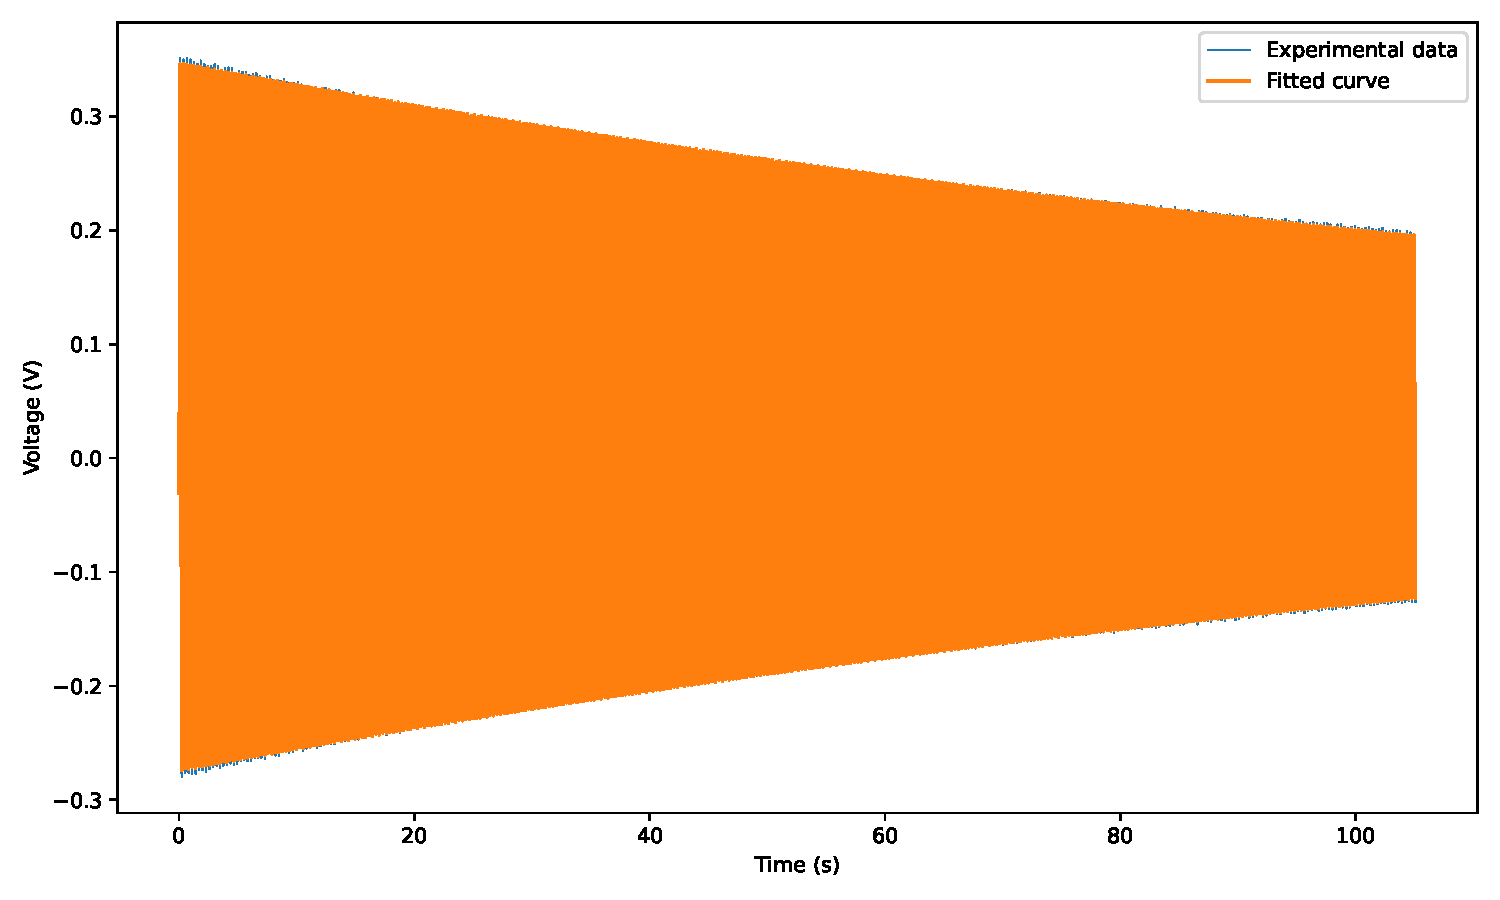
\includegraphics[width=0.6\textwidth]{results/group_01.pdf}
  \caption{\mbox {$d = 20 mm\ U(t) =0.31122805e^{-0.0063636816t}\cos\left(21.331951t-1.7873299\right)+0.036267269 \ R^2 = 0.99963484$}}
\end{figure}

\begin{figure}[H]
  \centering
  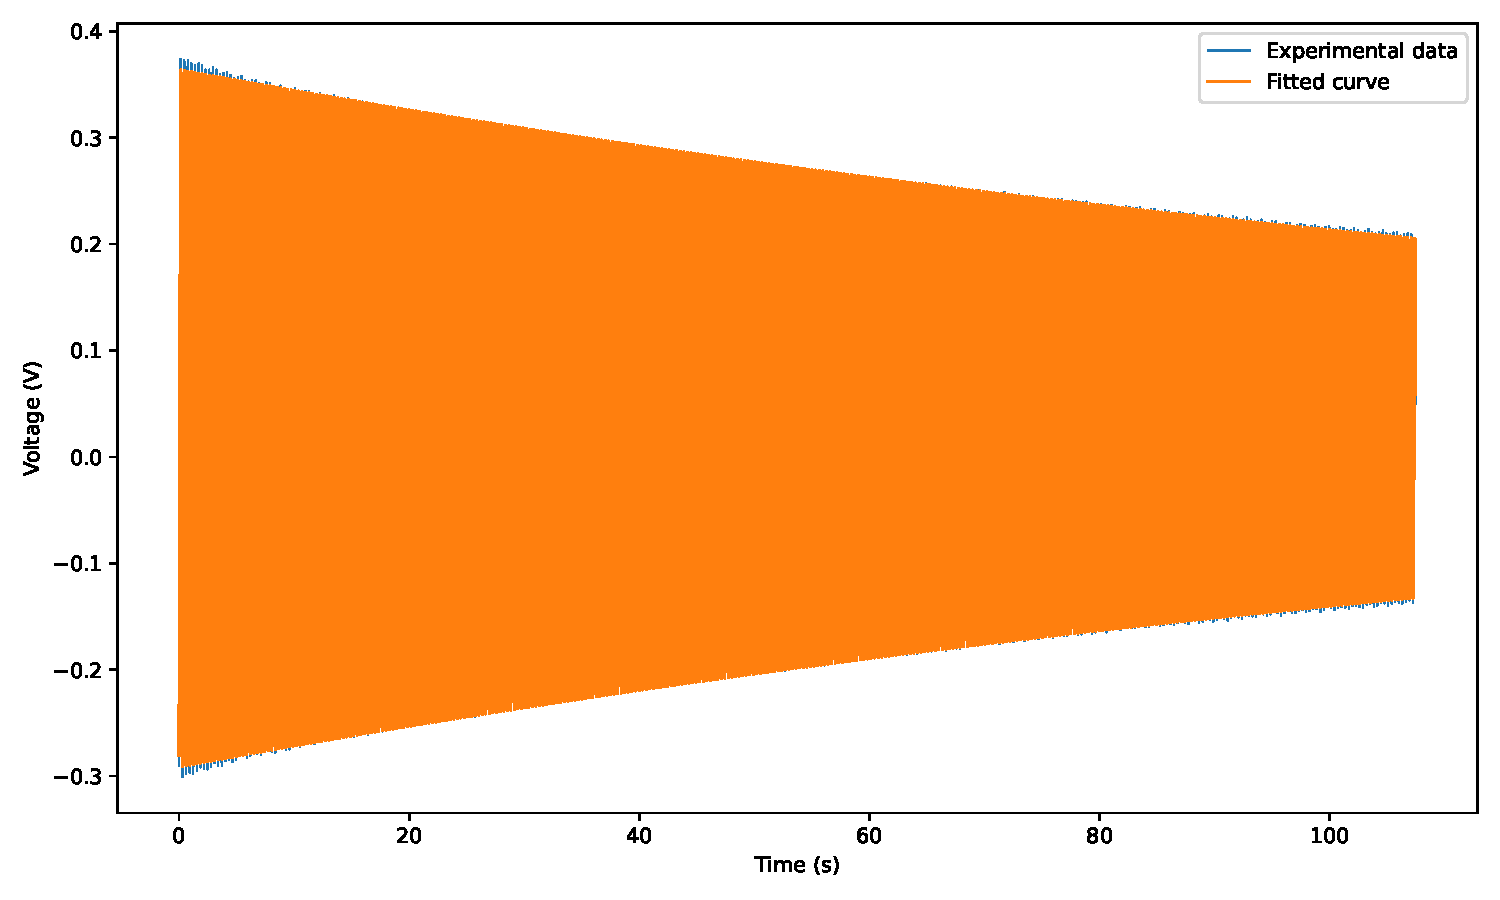
\includegraphics[width=0.6\textwidth]{results/group_02.pdf}
  \caption{\mbox{$d = 25mm\ U(t) =0.32813548e^{-0.0061645852t}\cos\left(20.268908t+3.4008697\right)+0.03618628 \ R^2 = 0.99957954$}}
\end{figure}

\begin{figure}[H]
  \centering
  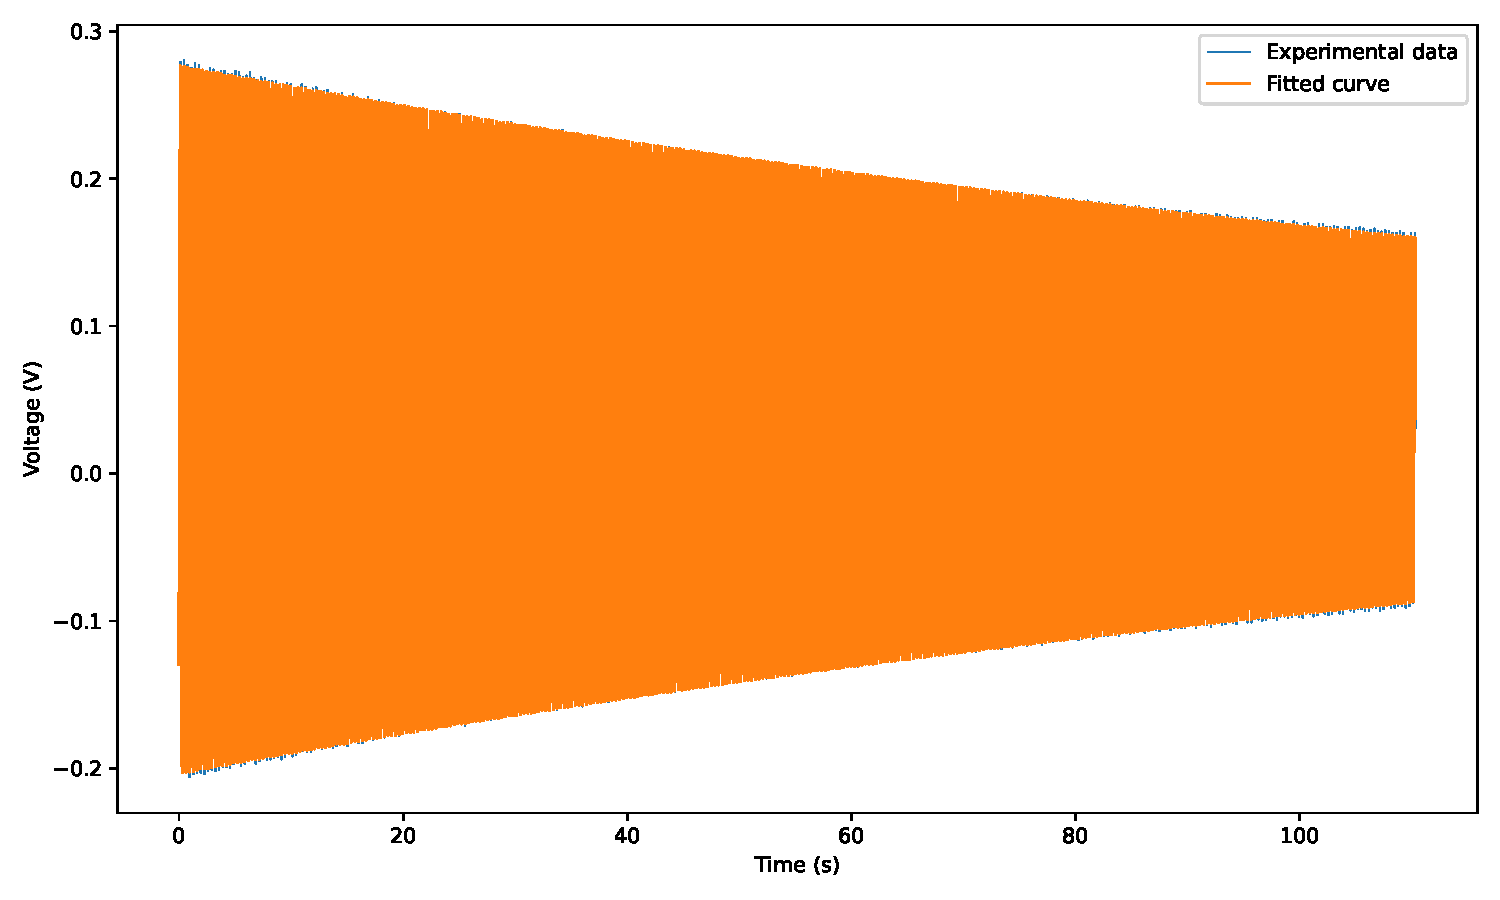
\includegraphics[width=0.6\textwidth]{results/group_03.pdf}
  \caption{\mbox{$d = 30mm\ U(t) =0.24021369e^{-0.0060099266t}\cos\left(19.164936t+3.9512331\right)+0.036386284\ R^2 = 0.99964596$}}
\end{figure}

\begin{figure}[H]
  \centering
  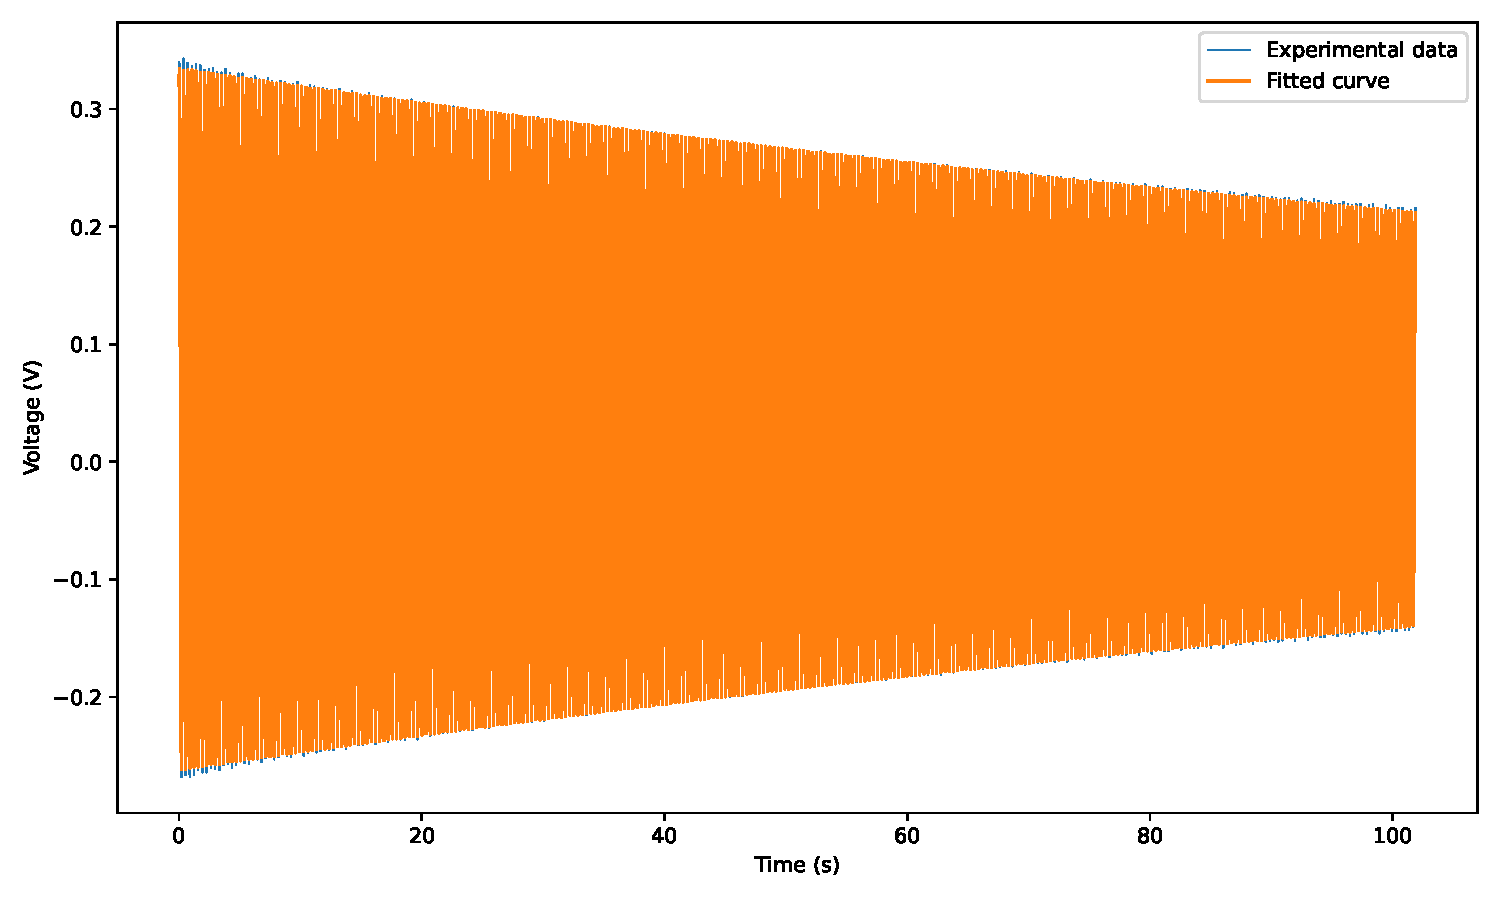
\includegraphics[width=0.6\textwidth]{results/group_04.pdf}
  \caption{\mbox{$d = 35mm\ U(t) =0.29837277e^{-0.0051893324t}\cos\left(18.073363t-0.31664223\right)+0.036228076\ R^2 = 0.99894511$}}
\end{figure}

\begin{figure}[H]
  \centering
  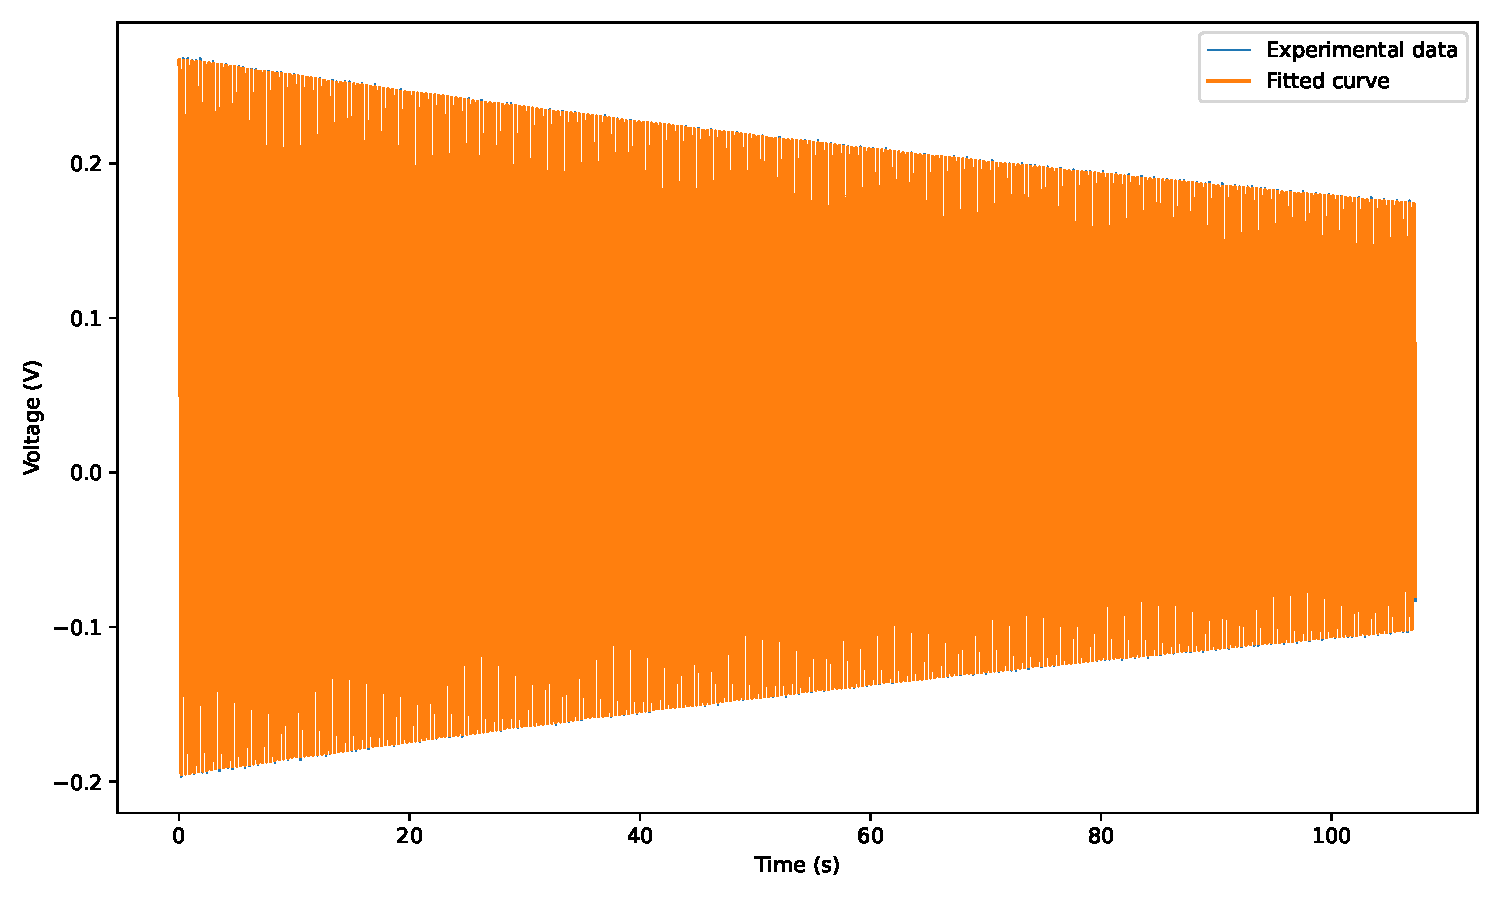
\includegraphics[width=0.6\textwidth]{results/group_05.pdf}
  \caption{\mbox{$d = 40mm\ U(t) =0.23175613e^{-0.0048443394t}\cos\left(17.008062t-0.094281856\right)+0.0361553\ R^2 = 0.99975478$}}
\end{figure}

\begin{figure}[H]
  \centering
  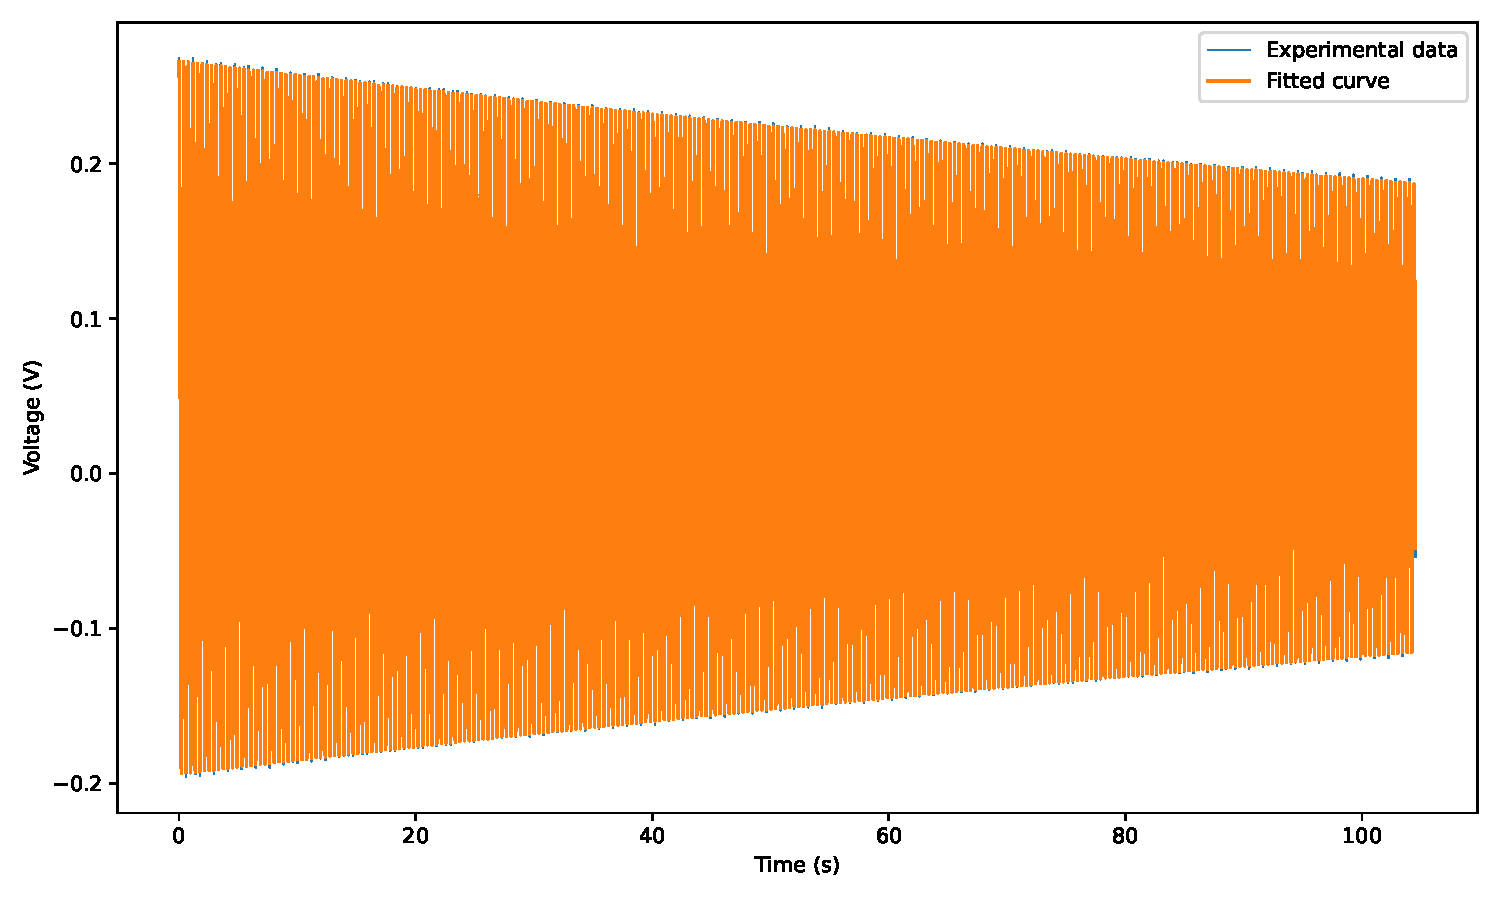
\includegraphics[width=0.6\textwidth]{results/group_06.pdf}
  \caption{\mbox{$d = 45mm\ U(t) =0.23033459e^{-0.0040168309t}\cos\left(16.007664t+0.049939726\right)+0.036059291\ R^2 = 0.99981743$}}
\end{figure}

\begin{figure}[H]
  \centering
  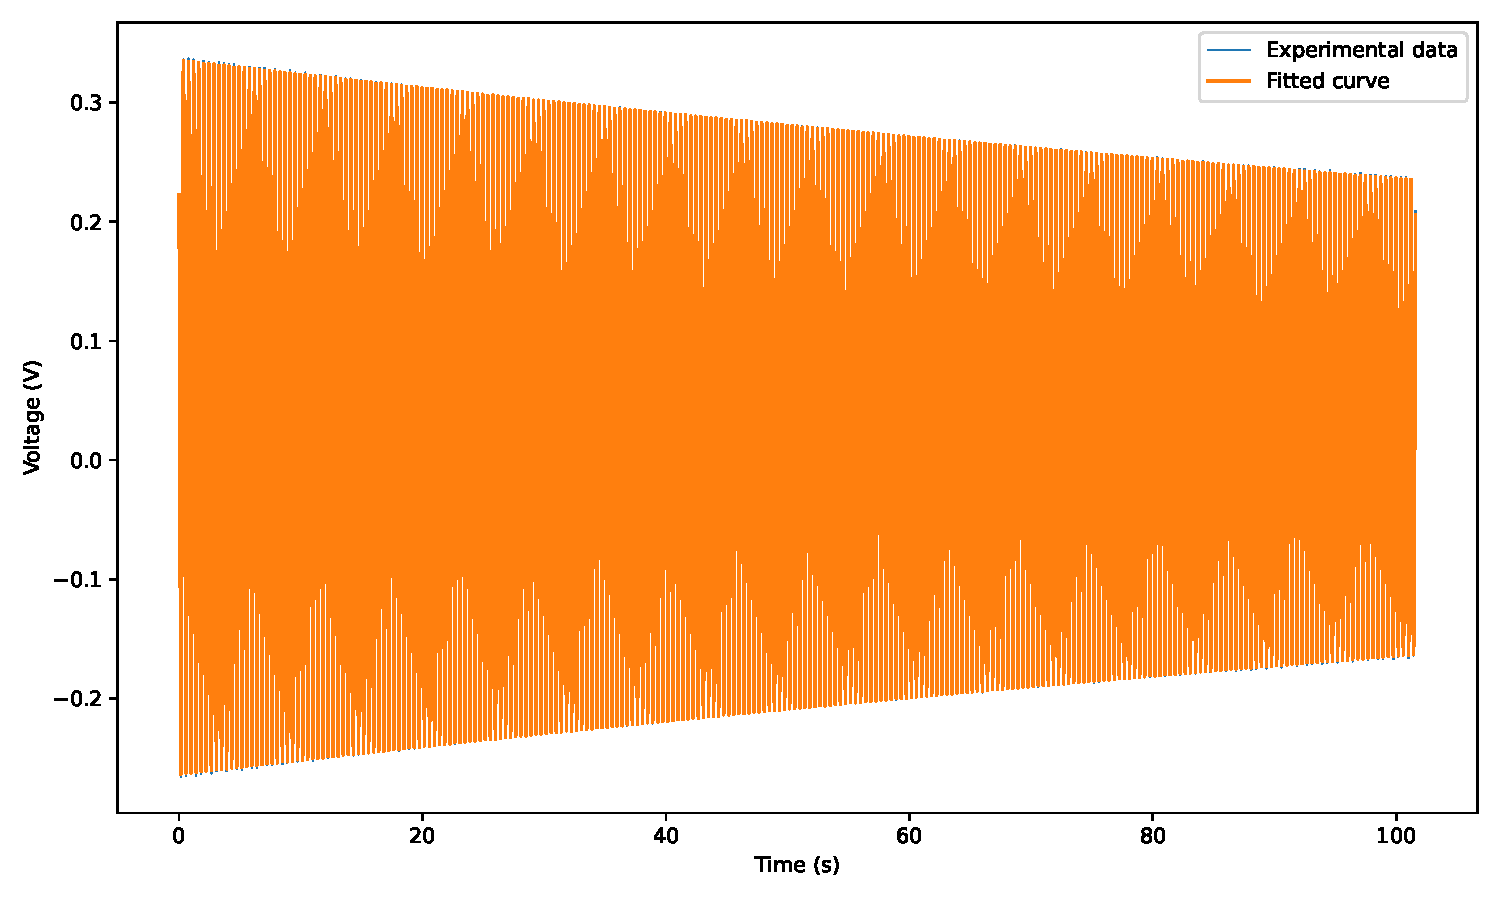
\includegraphics[width=0.6\textwidth]{results/group_07.pdf}
  \caption{\mbox{$d = 50mm\ U(t) =0.29984013e^{-0.0040235795t}\cos\left(15.075291t+0.89734709\right)+0.035936147\ R^2 = 0.99993768$}}
\end{figure}

\noindent 虽然这些图长得很像但确实不是一张图（）\newline
\noindent 根据图像和拟合结果，可以看到我们使用的阻尼振动模型确实是切合实际的

\subsection{测转动惯量}

\subsubsection{空载}

\begin{figure}[H]
  \centering
  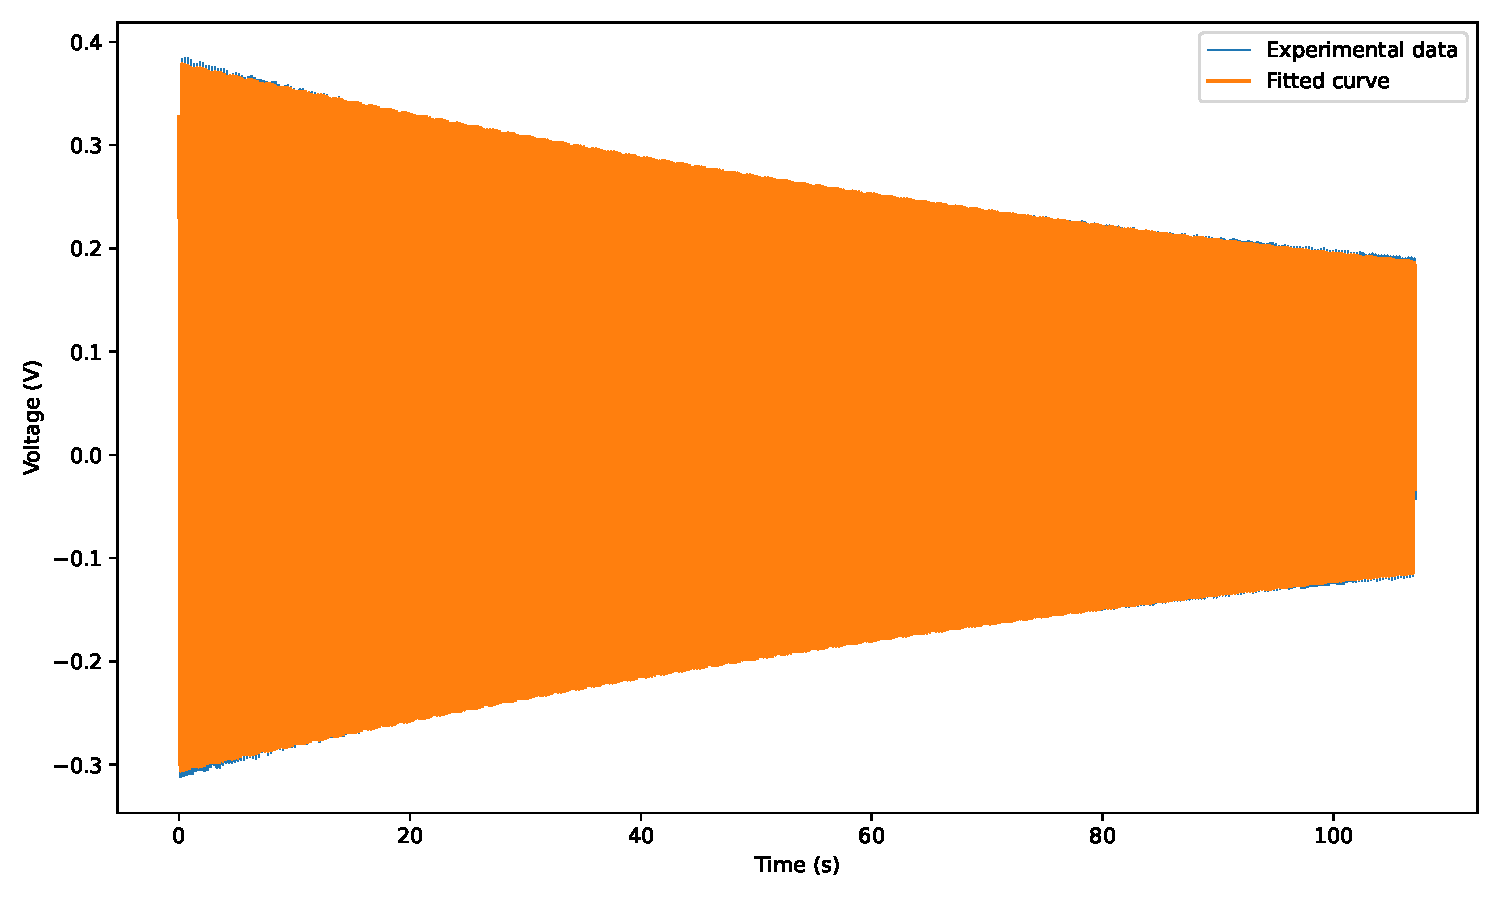
\includegraphics[width=0.6\textwidth]{results/group_08.pdf}
  \caption{\mbox{空载1\ $U(t) =0.34305996e^{-0.0076698148t}\cos\left(24.004059t+0.55511086\right)+0.036286971\ R^2 = 0.99946862$}}
\end{figure}

\begin{figure}[H]
  \centering
  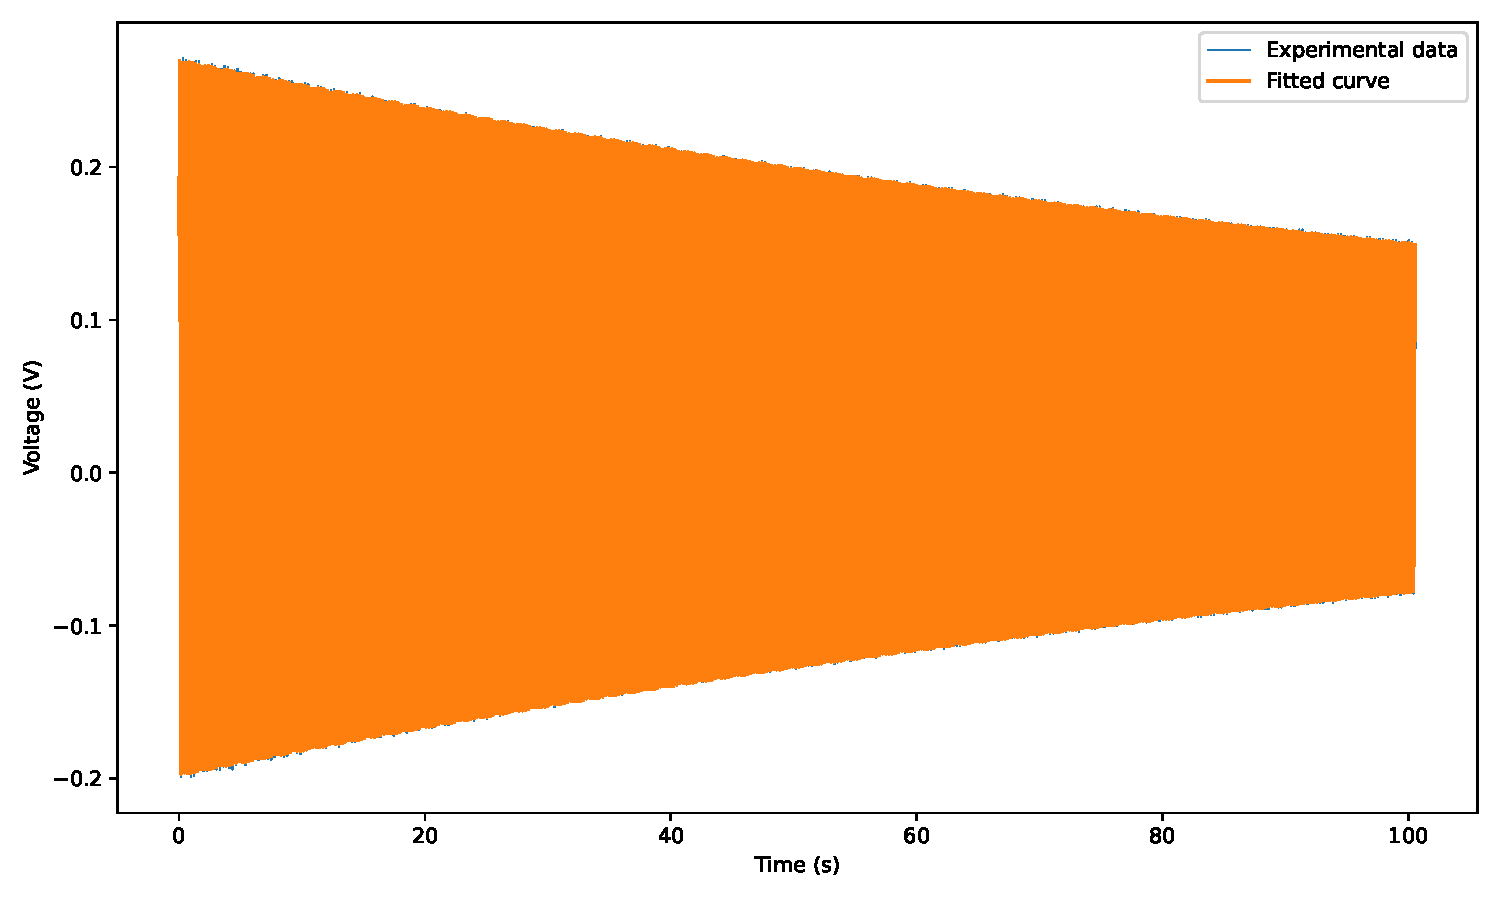
\includegraphics[width=0.6\textwidth]{results/group_12.pdf}
  \caption{\mbox{空载2\ $U(t) =0.23419206e^{-0.0071720096t}\cos\left(24.004827t-1.032905\right)+0.035928727\ R^2 = 0.99970213$}}
\end{figure}

\begin{figure}[H]
  \centering
  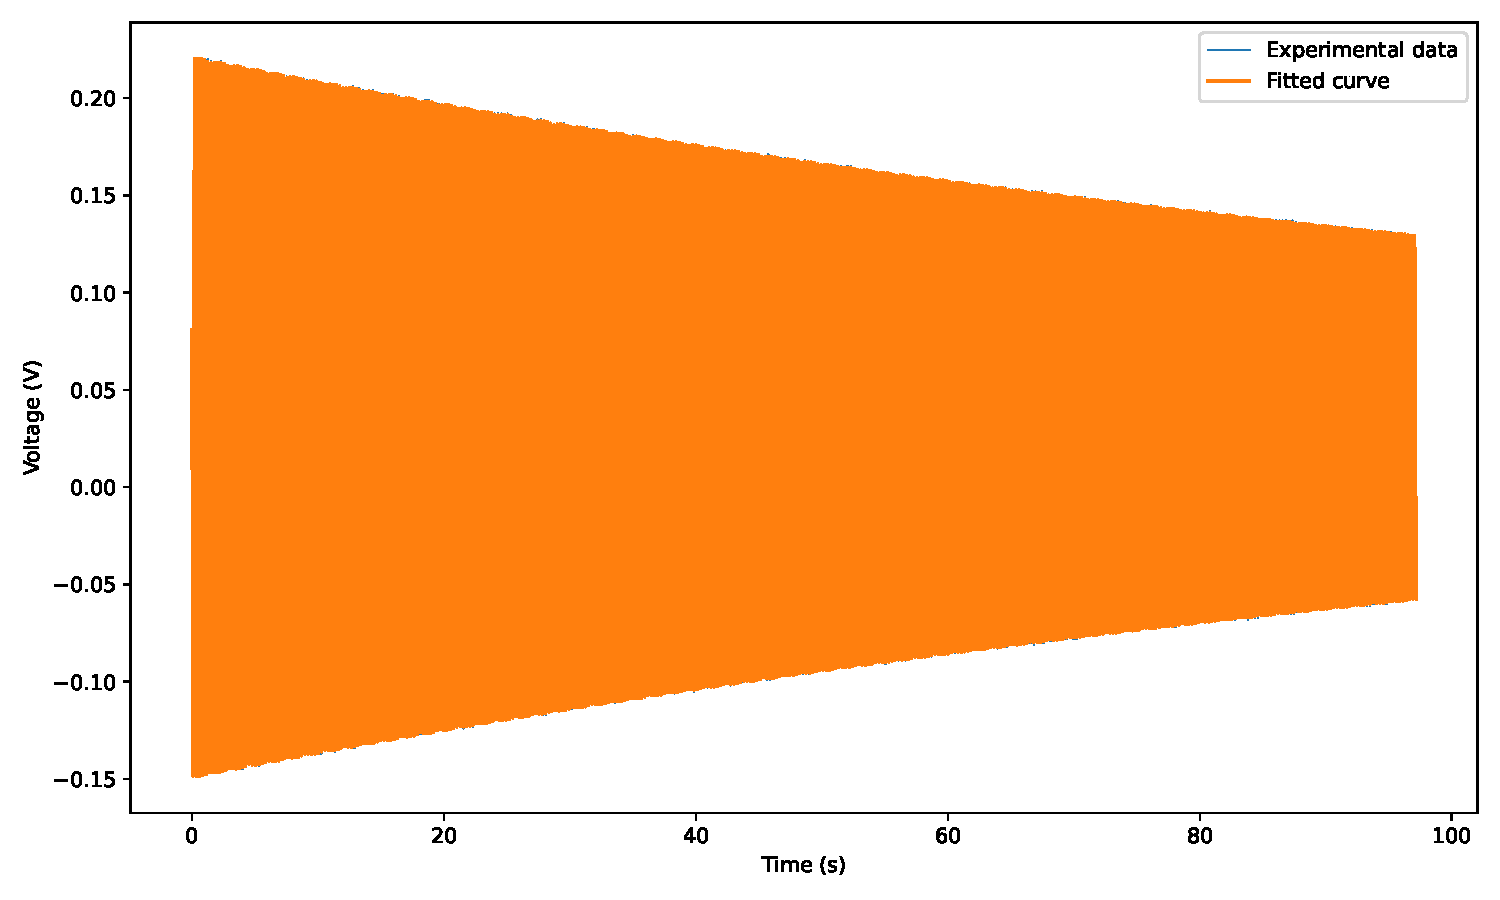
\includegraphics[width=0.6\textwidth]{results/group_13.pdf}
  \caption{\mbox{空载3\ $U(t)=0.18532096e^{-0.007018546t}\cos\left(24.006355t+1.3240911\right)+0.035843914\ R^2 = 0.99984109$}}
\end{figure}

\subsubsection{负载}

\begin{figure}[H]
  \centering
  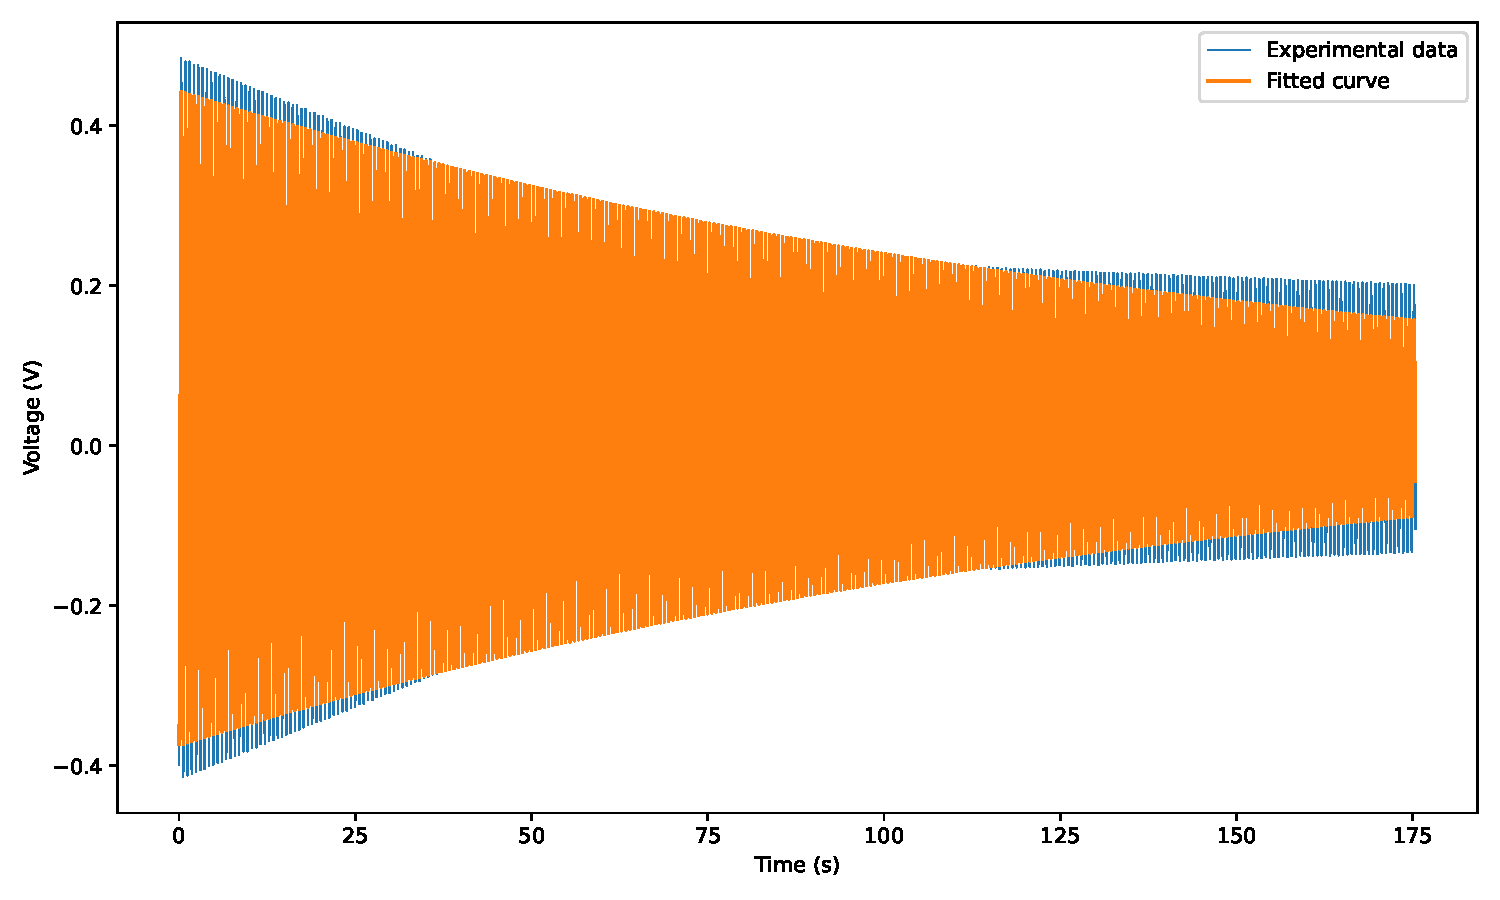
\includegraphics[width=0.6\textwidth]{results/group_09.pdf}
  \caption{\mbox{负载1\ $U(t)=0.40913817e^{-0.0068743692t}\cos\left(10.310037t+3.2454502\right)+0.034378556\ R^2 = 0.97503500$}}
\end{figure}

\begin{figure}[H]
  \centering
  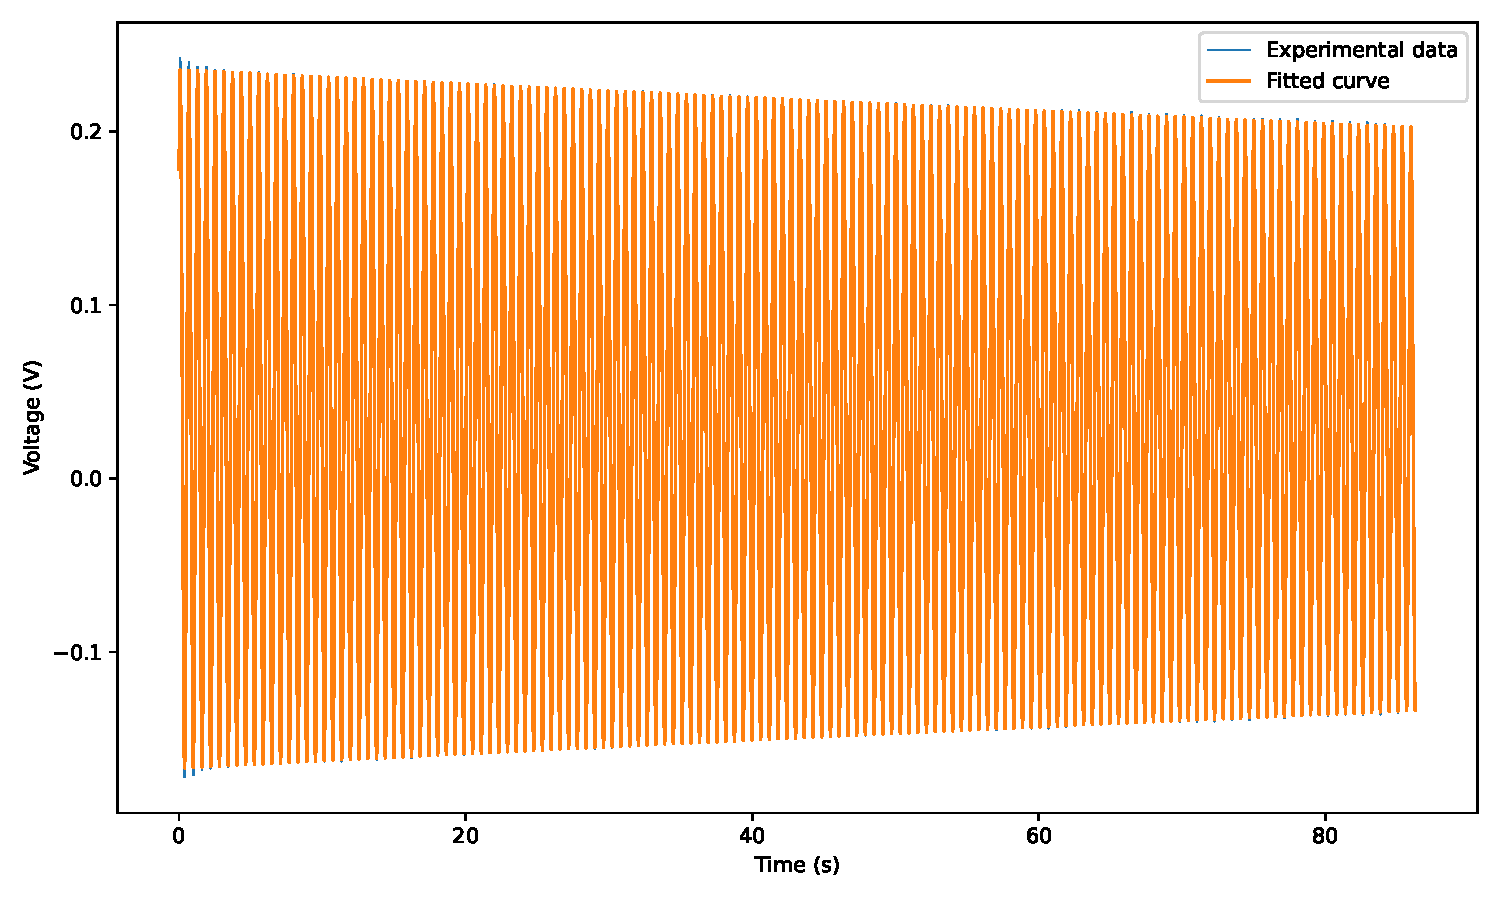
\includegraphics[width=0.6\textwidth]{results/group_10.pdf}
  \caption{\mbox{负载2\ $U(t)=0.20126225e^{-0.0020901044t}\cos\left(10.314196t-0.77648717\right)+0.03433489\ R^2 = 0.99995867$}}
\end{figure}

\begin{figure}[H]
  \centering
  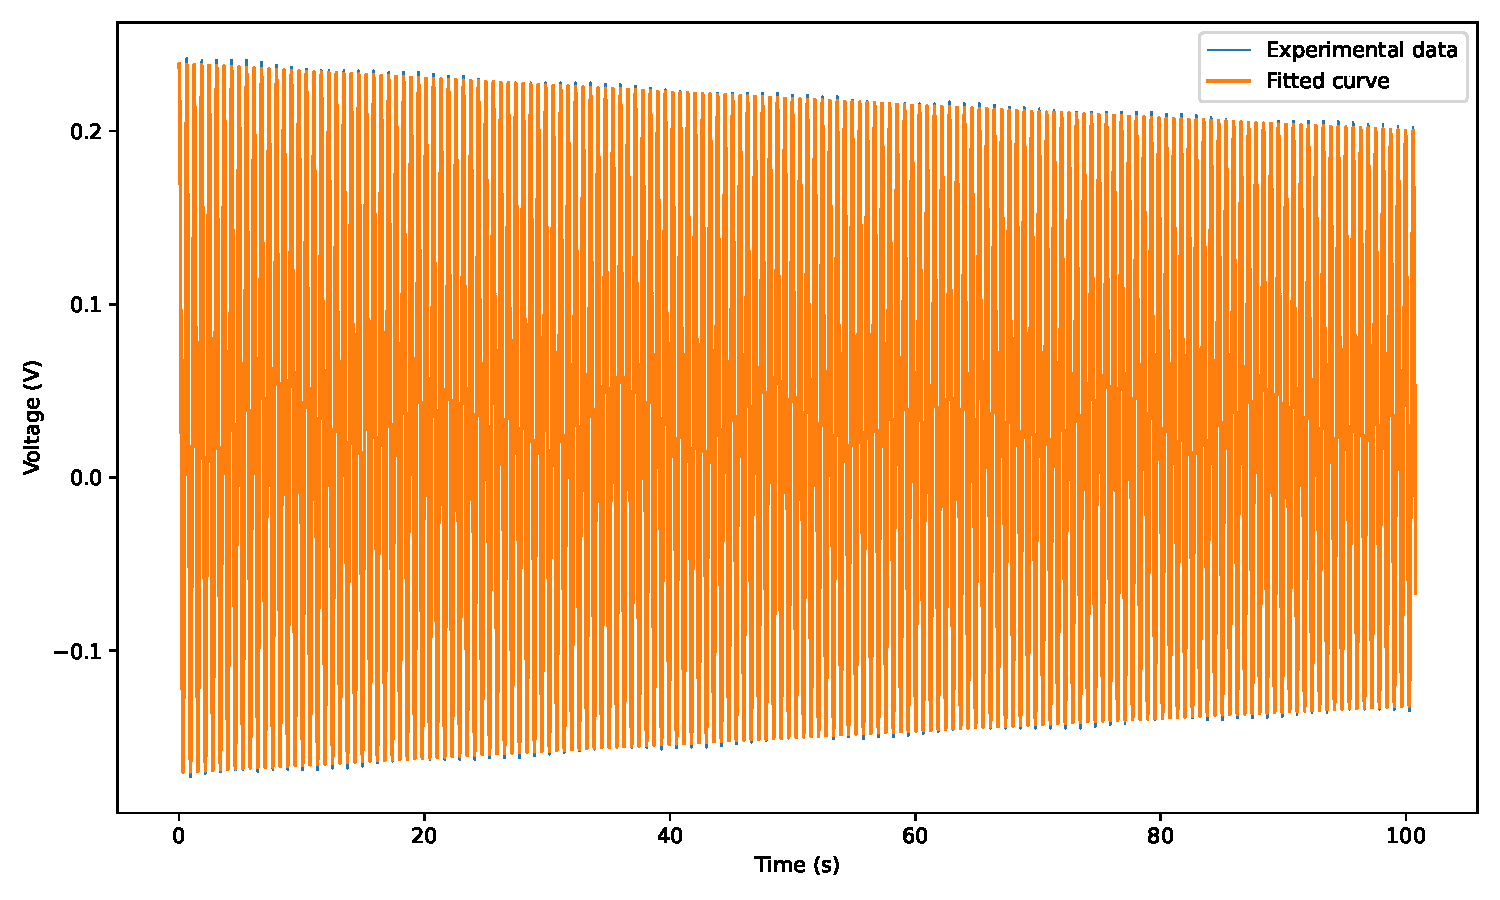
\includegraphics[width=0.6\textwidth]{results/group_11.pdf}
  \caption{\mbox{负载3\ $U(t) =0.20476132e^{-0.0020788117t}\cos\left(10.310639t-0.15395132\right)+0.034325519\ R^2 = 0.99970517$}}
\end{figure}

\section{误差分析与测量不确定度评定}

\subsection{不确定度的来源与评定方法}

本实验通过测量扭摆的振动角频率、扭丝几何尺寸及附加物体的质量，求得扭转系数、剪切模量和圆环转动惯量。测量不确定度分为通过重复测量或拟合残差进行统计评定的 A 类标准不确定度，以及依据仪器技术指标等非统计信息进行评定的 B 类标准不确定度。对于相互独立的两类不确定度，有
\begin{equation}
 u_c(x)=\sqrt{u_A^2(x)+u_B^2(x)}.
\end{equation}
以下数值采用原始测量数据，并取扭丝有效长度 $L=443.2\,\mathrm{mm}$、圆环内外径 $d_1=5.344\,\mathrm{cm}$、$d_2=7.660\,\mathrm{cm}$。由于尚未获得本次使用的各台仪器的校准证书，B 类评定采用普通教学实验室仪器的\textbf{参考规格}，并明确其假设；因此合成不确定度为条件性估计，并不包含所有可能的系统误差。

\subsection{A 类标准不确定度}

\subsubsection{扭丝直径}

扭丝直径的五次测量值分别为 $1.405$、$1.403$、$1.402$、$1.404$、$1.402\,\mathrm{mm}$，平均值为

\begin{equation}
 \overline D=\frac{1}{5}\sum_{i=1}^{5}D_i=1.4032\,\mathrm{mm}.
\end{equation}

平均值的 A 类标准不确定度采用贝塞尔公式：

\begin{equation}
 u_A(D)=\sqrt{\frac{\sum_{i=1}^{n}(D_i-\overline D)^2}{n(n-1)}}
 =5.831\times10^{-4}\,\mathrm{mm},\qquad n=5.
\end{equation}

\subsubsection{空载与负载角频率}

空载角频率的三次测量结果为 $24.0040$、$24.0048$、$24.0063\,\mathrm{rad/s}$；负载角频率的三次测量结果为 $10.3100$、$10.3141$、$10.3106\,\mathrm{rad/s}$。分别取平均值得到

\begin{equation}
 \overline\omega=24.00503\,\mathrm{rad/s},\qquad
 \overline\omega'=10.31157\,\mathrm{rad/s}.
\end{equation}

平均值的 A 类标准不确定度为

\begin{equation}
 u_A(\overline\omega)=\sqrt{\frac{\sum_{i=1}^{n}(\omega_i-\overline\omega)^2}{n(n-1)}}.
\end{equation}

计算得

\begin{equation}
 \begin{aligned}
 u_A(\overline\omega)&=6.741\times10^{-4}\,\mathrm{rad/s},\\
 u_A(\overline\omega')&=1.278\times10^{-3}\,\mathrm{rad/s}.
 \end{aligned}
\end{equation}

上述数据来自三次独立实验结果的离散程度，与单次阻尼振动非线性拟合参数协方差所给出的统计标准误差并不相同。

\subsubsection{直线拟合系数}

令 $x=d^2$、$y=1/\omega^2$，对七组测量值按照 $y=ax+b$ 进行普通最小二乘拟合，得到

\begin{equation}
 a=1.0489068\,\mathrm{s^2/m^2},\qquad
 b=0.001778117\,\mathrm{s^2},\qquad R^2=0.99999909.
\end{equation}

在拟合点纵坐标残差独立、同方差且横坐标误差可忽略的假设下，定义

\begin{equation}
 s_y=\sqrt{\frac{\sum_{i=1}^{n}(y_i-ax_i-b)^2}{n-2}},\qquad n=7,
\end{equation}

则斜率和截距的标准误差分别为

\begin{equation}
 \begin{aligned}
 u_A(a)&=\frac{s_y}{\sqrt{\sum_i(x_i-\overline x)^2}}
 =4.476\times10^{-4}\,\mathrm{s^2/m^2},\\
 u_A(b)&=s_y\sqrt{\frac1n+\frac{\overline x^2}{\sum_i(x_i-\overline x)^2}}
 =6.718\times10^{-7}\,\mathrm{s^2}.
 \end{aligned}
\end{equation}

由于 $a$、$b$ 来自同一次拟合，二者并不独立；后续计算 $I_0=2mb/a$ 时须考虑协方差。此外，上述拟合标准误差尚未考虑小球位置测量引起的横坐标不确定度。

\subsection{B 类标准不确定度}

若仪器最大允许误差为 $\pm\Delta$，并假设误差在该区间内服从矩形分布，则

\begin{equation}
 u_B=\frac{\Delta}{\sqrt3}.
\end{equation}

若仅考虑数字显示的量化误差，分辨率为 $q$，则对应的标准不确定度为 $q/\sqrt{12}$。准确度与分辨率不是同一概念，不应重复计入已被最大允许误差覆盖的误差来源。

\subsubsection{几何尺寸及质量测量}

参考普通实验室仪器的代表性规格：螺旋测微器最大允许误差 $\pm0.002\,\mathrm{mm}$，游标卡尺最大允许误差 $\pm0.03\,\mathrm{mm}$，电子天平线性误差 $\pm0.02\,\mathrm{g}$，钢卷尺在约 $0.44\,\mathrm{m}$ 量程下取参考最大允许误差 $\pm0.5\,\mathrm{mm}$。在矩形分布假设下得到

\begin{equation}
 \begin{aligned}
 u_B(D)&=0.001155\,\mathrm{mm},\\
 u_B(d_1)=u_B(d_2)&=0.01732\,\mathrm{mm},\\
 u_B(m)=u_B(M)&=0.01155\,\mathrm{g},\\
 u_B(L)&=0.2887\,\mathrm{mm}.
 \end{aligned}
\end{equation}

结合直径的重复测量结果：

\begin{equation}
 u_c(D)=\sqrt{(0.0005831)^2+(0.001155)^2}
 =0.001294\,\mathrm{mm},
\end{equation}

故

\begin{equation}
 D=(1.4032\pm0.0013)\,\mathrm{mm}.
\end{equation}

这些 B 类数值是参考仪器规格下的估算值，并非本实验实际器材的校准结果；仪器准确度、端点定位和小球位置等因素可能还需另外评定。

\subsubsection{PASCO 850 信号采集}

本实验通过 PASCO 850 接口采集电压--时间数据，再利用 Python 的 SciPy 库进行阻尼振动曲线拟合。对某种配置下参考的 ADC 量化步长 $q_U=2.5\,\mathrm{mV}$，若仅考虑矩形分布的量化误差，则

\begin{equation}
 u_{B,\mathrm{quant}}(U)=\frac{2.5}{\sqrt{12}}\,\mathrm{mV}
 \approx0.722\,\mathrm{mV}.
\end{equation}

但此数值仅代表\emph{该量化配置}的量化贡献，并非完整电压准确度，更不能直接作为角频率的不确定度。角频率是由电压信号拟合得到的参数，其不确定度还受采样时基、传感器噪声、模型偏差及拟合残差影响。由于缺少本次具体采集配置下的时基准确度，以下对角频率仅纳入已计算的 A 类贡献，未虚构独立的时基 B 类数值。


\subsection{间接测量量的合成标准不确定度}
以下暂假设相关输入量相互独立；斜率、截距联合传播时除外。

\subsubsection{扭转系数 $k$}

由 $a=2m/k$ 得 $k=2m/a$。取单颗小球质量 $m=0.03507\,\mathrm{kg}$，则

\begin{equation}
 k=\frac{2\times0.03507}{1.0489068}
 =0.0668696\,\mathrm{N\,m/rad}.
\end{equation}

在 $m$ 和 $a$ 独立的假设下，

\begin{equation}
 \frac{u_c(k)}{k}=\sqrt{\left(\frac{u_B(m)}m\right)^2+
 \left(\frac{u_A(a)}a\right)^2}.
\end{equation}

计算得

\begin{equation}
 u_c(k)\approx3.60\times10^{-5}\,\mathrm{N\,m/rad},
 \qquad k=(0.066870\pm0.000036)\,\mathrm{N\,m/rad}.
\end{equation}

此值没有包含小球位置误差、角频率时基误差及模型偏差的完整贡献。

\subsubsection{剪切模量 $\mu$}

圆截面扭丝的剪切模量为

\begin{equation}
 \mu=\frac{32kL}{\pi D^4}.
\end{equation}

取 $L=0.4432\,\mathrm m$、$D=1.4032\times10^{-3}\,\mathrm m$，得

\begin{equation}
 \mu=\frac{32\times0.0668696\times0.4432}
 {\pi(1.4032\times10^{-3})^4}
 =7.7866\times10^{10}\,\mathrm{Pa}.
\end{equation}

利用独立输入量的不确定度传播公式：

\begin{equation}
 \frac{u_c(\mu)}\mu=
 \sqrt{\left(\frac{u_c(k)}k\right)^2+
       \left(\frac{u_B(L)}L\right)^2+
       16\left(\frac{u_c(D)}D\right)^2}.
\end{equation}

其中系数 $16$ 源于 $\mu\propto D^{-4}$。代入前述标准不确定度，得到

\begin{equation}
 \frac{u_c(\mu)}\mu\approx0.378\%,\qquad
 u_c(\mu)\approx2.95\times10^8\,\mathrm{Pa}.
\end{equation}

故条件性估算结果为

\begin{equation}
 \boxed{\mu=(7.787\pm0.029)\times10^{10}\,\mathrm{Pa}}.
\end{equation}

\subsubsection{摆盘等效转动惯量 $I_0$}

由于 $b=I_0/k$，正确的关系为

\begin{equation}
 I_0=kb=\frac{2mb}{a}
 =1.18902\times10^{-4}\,\mathrm{kg\,m^2}.
\end{equation}

考虑拟合参数 $a$、$b$ 的协方差，并假设质量 $m$ 与拟合参数独立，则

\begin{equation}
 \begin{aligned}
 u_c^2(I_0)={}&\left(\frac{I_0}{m}\right)^2u_B^2(m)
 +\left(\frac{I_0}{a}\right)^2u_A^2(a)\\
 &+\left(\frac{2m}{a}\right)^2u_A^2(b)
 -2\frac{I_0}{a}\frac{2m}{a}\operatorname{Cov}(a,b).
 \end{aligned}
\end{equation}

利用七组数据的普通最小二乘协方差矩阵，得

\begin{equation}
 u_c(I_0)\approx1.01\times10^{-7}\,\mathrm{kg\,m^2},\qquad
 I_0\approx(1.1890\pm0.0010)\times10^{-4}\,\mathrm{kg\,m^2}.
\end{equation}

\subsubsection{圆环转动惯量测量值}

设 $\omega$ 为空载角频率、$\omega'$ 为负载角频率，则

\begin{equation}
 I_{\mathrm{mes}}=k\left(\frac1{\omega'^2}-\frac1{\omega^2}\right)
 =5.12853\times10^{-4}\,\mathrm{kg\,m^2}.
\end{equation}

在 $k$、$\omega$、$\omega'$ 互相独立的假设下：

\begin{equation}
 \begin{aligned}
 u^2(I_{\mathrm{mes}})={}&
 \left(\frac1{\omega'^2}-\frac1{\omega^2}\right)^2u_c^2(k)\\
 &+\left(\frac{2k}{\omega^3}\right)^2u_A^2(\overline\omega)
 +\left(\frac{2k}{\omega'^3}\right)^2u_A^2(\overline\omega').
 \end{aligned}
\end{equation}

代入得到

\begin{equation}
 u(I_{\mathrm{mes}})\approx3.17\times10^{-7}\,\mathrm{kg\,m^2},\qquad
 \boxed{I_{\mathrm{mes}}=(5.1285\pm0.0032)\times10^{-4}\,\mathrm{kg\,m^2}}.
\end{equation}

\subsubsection{圆环转动惯量理论值}

设圆环质量 $M=0.46816\,\mathrm{kg}$，内径 $d_1=0.05344\,\mathrm m$，外径 $d_2=0.07660\,\mathrm m$，则

\begin{equation}
 I_{\mathrm{cal}}=\frac M8(d_1^2+d_2^2)
 =5.10493\times10^{-4}\,\mathrm{kg\,m^2}.
\end{equation}

假设 $M$、$d_1$、$d_2$ 的误差独立，则

\begin{equation}
 \begin{aligned}
 u_c^2(I_{\mathrm{cal}})={}&
 \left(\frac{d_1^2+d_2^2}{8}\right)^2u_B^2(M)\\
 &+\left(\frac{Md_1}{4}\right)^2u_B^2(d_1)
 +\left(\frac{Md_2}{4}\right)^2u_B^2(d_2).
 \end{aligned}
\end{equation}

代入上述参考仪器指标，得到

\begin{equation}
 u_c(I_{\mathrm{cal}})\approx1.90\times10^{-7}\,\mathrm{kg\,m^2},\qquad
 \boxed{I_{\mathrm{cal}}=(5.1049\pm0.0019)\times10^{-4}\,\mathrm{kg\,m^2}}.
\end{equation}

\subsection{理论值与测量值比较}

圆环转动惯量测量值与理论值的相对误差为

\begin{equation}
 \delta=\frac{|I_{\mathrm{mes}}-I_{\mathrm{cal}}|}{I_{\mathrm{cal}}}\times100\%
 =\boxed{0.462\%}.
\end{equation}

绝对差值为

\begin{equation}
 |I_{\mathrm{mes}}-I_{\mathrm{cal}}|
 =2.36\times10^{-6}\,\mathrm{kg\,m^2}.
\end{equation}

若暂按两结果相互独立处理，差值的标准不确定度约为 $3.70\times10^{-7}\,\mathrm{kg\,m^2}$。实际差值约为其 $6.4$ 倍，提示当前纳入的不确定度来源不足以解释全部差异，尚可能存在装置安装、有效尺寸测量、几何偏心和拟合模型等系统性影响。这一比较依赖上述仪器规格及独立性假设，并非严格显著性检验。

\subsection{主要误差来源与改进措施}

1.扭丝直径和有效长度。由于 $\mu\propto D^{-4}$，扭丝直径的相对误差在一阶近似下会造成约四倍的剪切模量相对误差。应在不同位置和方向测量扭丝直径，关注截面圆度和仪器零点偏差。同时应精确定义并测量两夹持点之间的有效扭转长度，而不是仅取外露几何长度。

2.小球及圆环的安装位置。由于附加转动惯量与小球质心至转轴的距离平方有关，孔位误差、安装间隙或对称性不足会直接影响 $d^2$ 和线性拟合斜率。圆环若偏离转轴，按照平行轴定理会引入额外转动惯量。应尽可能保证小球对称、圆环同轴，并以实际质心位置作为几何测量依据。

3.阻尼与模型近似。真实扭摆还存在空气阻力、扭丝内耗及连接处摩擦。线性阻尼模型下，阻尼角频率 $\omega_d$ 与无阻尼固有角频率 $\omega_n$ 满足

\begin{equation}
 \omega_n^2=\omega_d^2+\beta^2.
\end{equation}

本实验拟合得到的 $\beta$ 约为 $0.002$--$0.008\,\mathrm{s^{-1}}$，而 $\omega_d$ 约为 $10$--$24\,\mathrm{rad/s}$；两者相差较大，故忽略 $\beta^2$ 对角频率关系的直接修正一般很小。但是，这并不能证明所有非线性阻尼或多模态振动均可忽略。

4.数字采集及拟合。使用 NumPy 的 FFT 估计角频率，使用 SciPy 的 Hilbert 变换估计振幅包络，再通过 \texttt{curve\_fit()} 进行非线性最小二乘优化。FFT 和 Hilbert 变换仅提供初始估计，最终参数仍受实际噪声及模型选择影响。多数实验组拟合决定系数较高，但负载第一组的 $R^2\approx0.9750$，明显低于其他组，应重点关注其残差、机械振动干扰及数据采集状态。较高 $R^2$ 并不能单独证明模型不存在系统偏差。

\subsection{不确定度结果汇总与结论}

\begin{table}[H]
\centering
\small
\caption{主要测量结果及已评定来源的标准不确定度}
\begin{tabular}{|l|l|l|}
\hline
物理量 & 测量或计算结果 & 标准不确定度估计 \\ \hline
扭丝直径 $D$ & $1.4032\,\mathrm{mm}$ & $0.00129\,\mathrm{mm}$ \\ \hline
扭转系数 $k$ & $0.0668696\,\mathrm{N\,m/rad}$ & $3.60\times10^{-5}\,\mathrm{N\,m/rad}$ \\ \hline
剪切模量 $\mu$ & $7.7866\times10^{10}\,\mathrm{Pa}$ & $2.95\times10^8\,\mathrm{Pa}$ \\ \hline
摆盘等效转动惯量 $I_0$ & $1.18902\times10^{-4}\,\mathrm{kg\,m^2}$ & $1.01\times10^{-7}\,\mathrm{kg\,m^2}$ \\ \hline
圆环测量值 $I_{\mathrm{mes}}$ & $5.12853\times10^{-4}\,\mathrm{kg\,m^2}$ & $3.17\times10^{-7}\,\mathrm{kg\,m^2}$ \\ \hline
圆环理论值 $I_{\mathrm{cal}}$ & $5.10493\times10^{-4}\,\mathrm{kg\,m^2}$ & $1.90\times10^{-7}\,\mathrm{kg\,m^2}$ \\ \hline
\end{tabular}
\end{table}

综上，在采用参考仪器准确度并假设所列输入量满足相应独立性条件时，得到

\begin{equation}
 \boxed{\mu=(7.787\pm0.029)\times10^{10}\,\mathrm{Pa}},
\end{equation}

\begin{equation}
 \boxed{I_{\mathrm{mes}}=(5.1285\pm0.0032)\times10^{-4}\,\mathrm{kg\,m^2}}.
\end{equation}

测量值与理论值的相对误差约为 $0.462\%$。剪切模量的不确定度对扭丝直径较为敏感，圆环转动惯量还受到安装同轴度、角频率拟合和扭转系数估计的影响。表中均为已纳入来源的标准不确定度估计，并非依据实际器材校准结果完成的全面不确定度预算。

\section{附录}

\subsection{拟合代码}

\subsubsection{线性拟合代码}

\lstinputlisting[language=Python,frame=single,breaklines=true]{fit2.py}

\subsubsection{阻尼振动拟合代码}

\lstinputlisting[language=Python,frame=single,breaklines=true]{fit.py}

\subsection{数据}

原始数据见：\\

\url{https://github.com/alizeisnotalize/physics-experiment/TorsionPendulum}\\


看了就要给我star哦～

\
\begin{figure}[H]
  \centering
  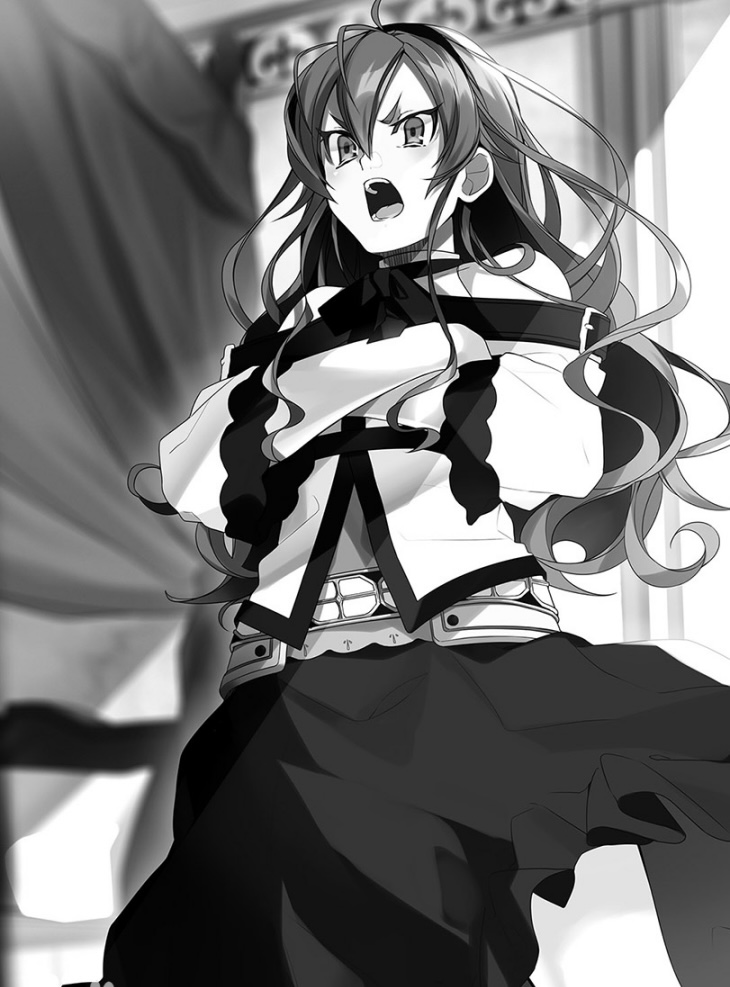
\includegraphics[width=0.75\textwidth]{艾莉丝.jpg}
  \caption{既然还有位置那就放张超可爱的艾莉丝吧}
\end{figure}
\end{document}